% Copyright (c) Meta Platforms, Inc. and affiliates.

\documentclass[twoside,11pt]{article}

\usepackage[nohyperref]{jmlr2e}
% Copyright (c) Meta Platforms, Inc. and affiliates.
%%%%% NEW MATH DEFINITIONS %%%%%

\usepackage{amsmath,amsfonts,bm,mathtools,amssymb}

\def\ceil#1{\lceil #1 \rceil}
\def\floor#1{\lfloor #1 \rfloor}
\def\1{\bm{1}}

\def\gA{{\mathcal{A}}}
\def\gB{{\mathcal{B}}}
\def\gC{{\mathcal{C}}}
\def\gD{{\mathcal{D}}}
\def\gE{{\mathcal{E}}}
\def\gF{{\mathcal{F}}}
\def\gG{{\mathcal{G}}}
\def\gH{{\mathcal{H}}}
\def\gI{{\mathcal{I}}}
\def\gJ{{\mathcal{J}}}
\def\gK{{\mathcal{K}}}
\def\gL{{\mathcal{L}}}
\def\gM{{\mathcal{M}}}
\def\gN{{\mathcal{N}}}
\def\gO{{\mathcal{O}}}
\def\gP{{\mathcal{P}}}
\def\gQ{{\mathcal{Q}}}
\def\gR{{\mathcal{R}}}
\def\gS{{\mathcal{S}}}
\def\gT{{\mathcal{T}}}
\def\gU{{\mathcal{U}}}
\def\gV{{\mathcal{V}}}
\def\gW{{\mathcal{W}}}
\def\gX{{\mathcal{X}}}
\def\gY{{\mathcal{Y}}}
\def\gZ{{\mathcal{Z}}}

\def\sA{{\mathbb{A}}}
\def\sB{{\mathbb{B}}}
\def\sC{{\mathbb{C}}}
\def\sD{{\mathbb{D}}}
% Don't use a set called E, because this would be the same as our symbol
% for expectation.
\def\sF{{\mathbb{F}}}
\def\sG{{\mathbb{G}}}
\def\sH{{\mathbb{H}}}
\def\sI{{\mathbb{I}}}
\def\sJ{{\mathbb{J}}}
\def\sK{{\mathbb{K}}}
\def\sL{{\mathbb{L}}}
\def\sM{{\mathbb{M}}}
\def\sN{{\mathbb{N}}}
\def\sO{{\mathbb{O}}}
\def\sP{{\mathbb{P}}}
\def\sQ{{\mathbb{Q}}}
\def\sR{{\mathbb{R}}}
\def\sS{{\mathbb{S}}}
\def\sT{{\mathbb{T}}}
\def\sU{{\mathbb{U}}}
\def\sV{{\mathbb{V}}}
\def\sW{{\mathbb{W}}}
\def\sX{{\mathbb{X}}}
\def\sY{{\mathbb{Y}}}
\def\sZ{{\mathbb{Z}}}


% \newcommand{\E}{\mathbb{E}}
\DeclareMathOperator{\E}{\mathbb{E}}
\DeclareMathOperator{\HH}{\mathbb{H}}
\DeclareMathOperator{\Var}{\rm{Var}}
\newcommand{\Ls}{\mathcal{L}}
\newcommand{\R}{\mathbb{R}}
\newcommand{\D}{\mathrm{D}}

\DeclareMathOperator*{\argmax}{arg\,max}
\DeclareMathOperator*{\argmin}{arg\,min}
\DeclareMathOperator*{\minimize}{minimize}
\DeclareMathOperator*{\maximize}{maximize}
\DeclareMathOperator*{\subjectto}{subject\;to}
\DeclareMathOperator*{\st}{s.t.}

\DeclarePairedDelimiterX{\infdivx}[2]{(}{)}{%
  #1\;\delimsize|\delimsize|\;#2%
}
\newcommand{\kl}[2]{\ensuremath{{\rm D}_{\rm KL}\infdivx{#1}{#2}}\xspace}
\newcommand{\dist}[2]{\ensuremath{{\rm D}\infdivx{#1}{#2}}\xspace}

\DeclareMathOperator{\sign}{sign}
\DeclareMathOperator{\Tr}{Tr}
\DeclareMathOperator{\ELBO}{ELBO}
\let\ab\allowbreak

\newcommand{\ftrans}{\ensuremath{f^{\mathrm{trans}}}}
\newcommand{\fodec}{\ensuremath{f^{\mathrm{odec}}}}
\newcommand{\frew}{\ensuremath{f^{\mathrm{rew}}}}
\newcommand{\fdec}{\ensuremath{f^{\mathrm{dec}}}}


\newcommand{\xinit}{{x_{\rm init}}}
\newcommand{\uinit}{{u_{\rm init}}}
\newcommand{\piold}{{\pi_{\theta_{\rm old}}}}

\newcommand{\defeq}{\vcentcolon=}
\newcommand{\eqdef}{=\vcentcolon}

\newcommand{\gradupdate}{\ensuremath{\mathrm{grad\_update}}}

\newcommand{\stopgrad}[2]{ \underset{\tiny\mathbf{stop}(#2)}{\left\llbracket{}#1\right\rrbracket{}} }


\usepackage[utf8]{inputenc} % allow utf-8 input
\usepackage[T1]{fontenc}    % use 8-bit T1 fonts
\usepackage{url}            % simple URL typesetting
\usepackage{booktabs}       % professional-quality tables
\usepackage{amsfonts}       % blackboard math symbols
\usepackage{nicefrac}       % compact symbols for 1/2, etc.
\usepackage{microtype}      % microtypography
\usepackage{enumitem}
\usepackage{slantsc}
\usepackage{caption}

\renewcommand\eminnershape{\itshape\scshape}

\usepackage{xcolor}
\definecolor{linkcolor}{RGB}{168, 141, 201}
\usepackage[
colorlinks=true,allcolors=linkcolor,pageanchor=true,
plainpages=false,pdfpagelabels,bookmarks,bookmarksnumbered,
backref=page
]{hyperref}

\renewcommand*{\backref}[1]{}
\renewcommand*{\backrefalt}[4]{%
  \ifcase #1 \or (Cited on page~#2.)
  \else (Cited on pages~#2.)
  \fi%
}


\usepackage[nameinlink]{cleveref}
\Crefname{equation}{Eq.}{Eqs.}

\usepackage{xspace}
\newcommand{\eg}{e.g.\xspace}
\newcommand{\ie}{i.e.\xspace}

\newcommand\pro{\item[$+$]}
\newcommand\con{\item[$-$]}

\usepackage{wrapfig}
\usepackage{tikz}
\usetikzlibrary{arrows.meta, arrows, calc, matrix}

\setlength\tabcolsep{4 pt}

\newcommand{\cblock}[3]{
  \hspace{-1.5mm}
  \begin{tikzpicture}
    [
    node/.style={square, minimum size=10mm, thick, line width=0pt},
    ]
    \node[fill={rgb,255:red,#1;green,#2;blue,#3}] () [] {};
  \end{tikzpicture}%
}

\jmlrheading{Z}{2022}{XX-YY}{1/22}{XX/YY}{amos2022}{Brandon Amos}

\ShortHeadings{Tutorial on amortized optimization}{Amos}
\firstpageno{1}

\begin{document}

\title{Tutorial on amortized optimization for
learning to optimize over continuous domains}
\author{\name Brandon Amos \email bda@fb.com \\
  \addr Facebook AI Research, Meta}
\editor{}

\maketitle

\begin{abstract}
  Optimization is a ubiquitous modeling tool and is often
  deployed in settings which repeatedly solve similar
  instances of the same problem.
  Amortized optimization methods use learning to predict
  the solutions to problems in these settings.
  This leverages the shared structure between
  similar problem instances.
  In this tutorial, we will discuss the key design choices
  behind amortized optimization,
  roughly categorizing 1) models into fully-amortized
  and semi-amortized approaches, and 2) learning methods
  into regression-based and objective-based.
  We then view existing applications through these
  foundations to draw connections between them,
  including for manifold optimization, variational inference,
  sparse coding, meta-learning, control, reinforcement learning,
  convex optimization, and deep equilibrium networks.
  This framing enables us easily see, for example, that the
  amortized inference in variational autoencoders is conceptually
  identical to value gradients in control and reinforcement
  learning as they both use fully-amortized models with
  an objective-based loss. \\

  \noindent The source code for this tutorial is available at:
  \begin{center}
  \url{https://github.com/facebookresearch/amortized-optimization-tutorial}
  \end{center}
\end{abstract}

\newpage
\setcounter{tocdepth}{2}
\tableofcontents

\newpage
\section{Introduction}
\begin{wrapfigure}{r}{1.8in}
\vspace{-4mm}
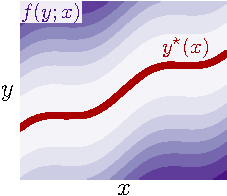
\includegraphics[width=\linewidth]{fig/opt.pdf}\vspace{-2mm}
\captionsetup{font={footnotesize}}
\caption{Illustration of \cref{eq:opt}.}
\vspace{-2mm}
\end{wrapfigure}
We study the use of machine learning
to improve repeated solves of optimization problems
\begin{equation}
  y^\star(x) \in \argmin_y f(y; x),
  \label{eq:opt}
\end{equation}
where the \emph{non-convex} objective
$f: \gY\times \gX\rightarrow \R$
takes a \emph{context} or \emph{parameterization}
$x\in\gX$ which can be continuous or discrete,
and the \emph{continuous, unconstrained domain} of
the problem is $y\in\gY=\R^n$.
A \emph{solution} $y^\star(x)\in\gY$, which we will often
assume to be unique, is implicitly defined via
the optimization procedure and captures the similarities
between problems with different contexts.
Parametric optimization problems of this form
have been studied for decades
\citep{bank1982non,fiacco1990sensitivity,shapiro2003sensitivity,klatte2006nonsmooth,bonnans2013perturbation,still2018lectures,fiacco2020mathematical}
with a large focus on sensitivity analysis.
This general formulation captures many
tasks arising in physics, engineering, mathematics, control,
and machine learning.
For example, when controlling a continuous robotic system,
$\gX$ is the space of \emph{observations} or \emph{states},
the domain $\gY\defeq \gU$ is the \emph{control space},
and $f(u; x)\defeq -Q(u, x)$ is the \emph{control cost}
or the negated \emph{Q-value} of the state-action tuple $(x,u)$.
For every encountered state $x$, the system is controlled
by solving an optimization problem in the form of \cref{eq:opt}.

Optimization problems such as \cref{eq:opt} quickly become a
computational bottleneck in systems.
\Cref{eq:opt} often does not have a closed-form
analytic solution and is instead solved with
approximate numerical methods which iteratively
search for the solution.
This computational problem has led to many specialized
solvers that leverage domain-specific insights to
deliver fast solves. Specialized algorithms are
especially prevalent in convex optimization methods for
linear programming, quadratic programming, cone programming,
and control and use theoretical insights of the problem
structure to bring empirical gains of computational
improvements and improved convergence.

\textbf{Overview.} This is a tutorial on \emph{amortized optimization},
which is the use of machine learning and statistical
methods to augment and computationally speed up
optimization methods which solve \cref{eq:opt}.
We focus on the modeling and learning tools necessary for
building learning-augmented solvers and extensions of
classical optimization methods.
Amortized optimization methods are capable of
significantly surpassing the convergence bounds derived
for classical algorithms
\emph{on a focused subset of problems}
because the convergence bounds are typically for worst-
or average-case analysis.
My goal in writing this is to explore a unified perspective
of modeling approaches of amortized optimization to help draw
connections between applications, for example between
amortized variational inference, meta-learning,
and policy learning for control and reinforcement learning.
I also connect to selected applications
in manifold optimization, sparse coding, convex optimization,
and deep equilibrium networks and discuss extensions
and other applications beyond the scope here.

\begin{figure}[t]
  \centering
  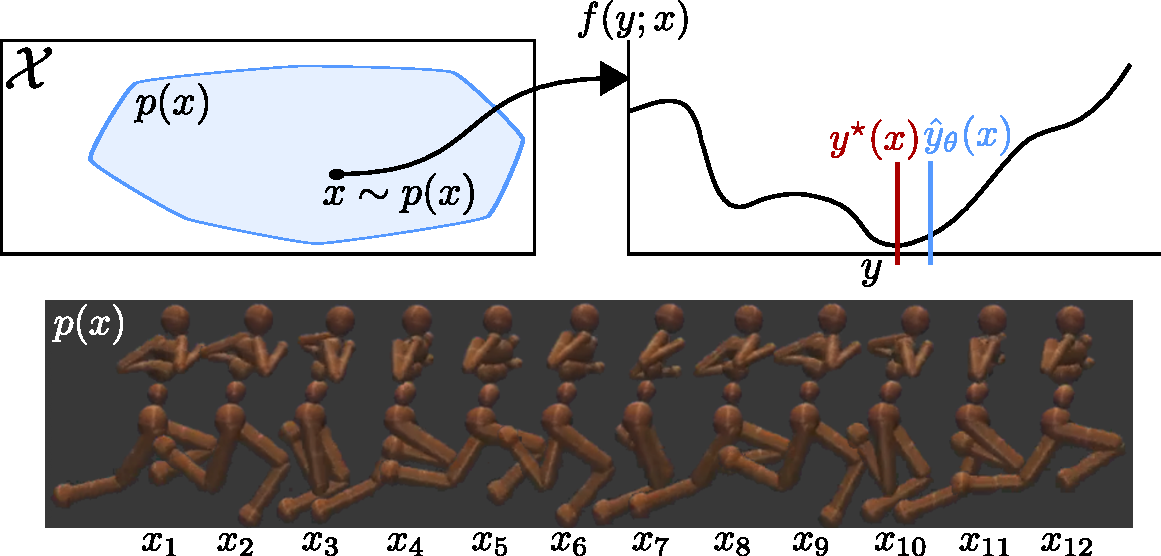
\includegraphics[width=\textwidth]{fig/overview.pdf}
  \caption{An amortized optimization method learns
    a model $\hat y_\theta$ to predict the minimum
    of an \emph{objective} $f(y;x)$ to a parameterized
    optimization problem, as in \cref{eq:opt},
    which depends on a \emph{context} $x$.
    For example, in control,
    the context space $\gX$ is the state space of the system,
    the domain $\gY\defeq\gU$ is the control space,
    the cost (or negated value) of a state-action
    pair is $f(u; x)\defeq -Q(x,u)$, and the state distribution is $p(x)$.
    For an encountered state $x$,
    many reinforcement learning policies $\pi_\theta(x)\defeq\hat y_\theta(x)$
    amortize the solution to the underlying control problem
    with true solution $y^\star(x)$.
    This humanoid policy was obtained with the model-based
    stochastic value gradient in \citet{amos2021model}.
  }
  \label{fig:overview}
\end{figure}

% \newpage
\section{Amortized optimization foundations for learning to optimize}
The machine learning, statistics, and optimization
communities are exploring methods of \emph{learning
to optimize} to obtain fast solvers for \cref{eq:opt}.
We will refer to these methods as \emph{amortized optimization}
as they \emph{amortize} the cost of solving the
optimization problems across many contexts to approximate
the solution mapping $y^\star$.
Amortized optimization is promising because in many applications,
there are significant correlations and structure between the
solutions which show up in $y^\star$ that a model can learn.
We follow \citet{shu2017amortized} for defining the core
foundation of amortized optimization as:

\begin{definition}
  An \emph{amortized optimization method} to solve \cref{eq:opt}
  can be represented by
  $\gA\defeq (f, \gY, \gX, p(x), \hat y_\theta, \gL)$,
  where
  $f: \gY\times\gX \rightarrow \R$ is the
  unconstrained \emph{objective} to optimize,
  $\gY$ is the \emph{domain},
  $\gX$ is the \emph{context space},
  $p(x)$ is the \emph{probability distribution over contexts} to optimize,
  $\hat y_\theta: \gX\rightarrow \gY$ is the \emph{amortization model}
  parameterized by $\theta$
  which is learned by optimizing a \emph{loss}
  defined on all the components
  $\gL(f, \gY, \gX, p(x), \hat y_\theta)$.
  \label{def:amor}
\end{definition}

The objective $f$ and domain $\gY$ arise from
the problem setting along with the context space
$\gX$ and distribution over it $p(x)$, and
the remaining definitions of the model
$\hat y_\theta$ and loss $\gL$ are application-specific
design decisions that \cref{sec:model,sec:learning}
opens up.
\Cref{fig:overview} illustrates these components.
The model $\hat y_\theta$ solves the solution mapping
$y^\star$ simultaneously for all contexts.
We also usually (informally) assume the solution mapping
$y^\star$ to be almost-everywhere smooth and well-behaved.
The best modeling approach is an open research topic
as there are many tradeoffs,
and many specialized insights from the application domain
can significantly improve the performance.
The generalization capacity along with the model's
convergence guarantees are challenging topics
which \cref{sec:generalization} covers in more detail.

\textbf{Origins of the term ``amortization'' for optimization.}
The word ``amortization'' generally means to spread out costs and
thus ``amortized optimization'' usually means to spread out
computational costs of the optimization process.
The term originated in the variational inference community
for inference optimization
\citep{kingma2013auto,rezende2014stochastic,stuhlmuller2013learning,gershman2014amortized,webb2017faithful,ravi2018amortized,cremer2018inference,wu2020meta},
and is used more generally in
\citep{xue2020amortized,sercu2021neural,xiao2021amortized}.
\citet[p.~28]{marino2021learned} give further background on the
origins and uses of amortization.

\textbf{Conventions and notation.}
The context space $\gX$ represents the
sample space of a probability space that
the distribution $p(x)$ is defined on,
assuming it is Borel if not otherwise specified.
For a function $f: \R^n\rightarrow\R$ in standard Euclidean space,
we denote the \emph{gradient} at a point $\bar x$
with $\nabla_x f(\bar x)\in \R^n$
and the \emph{Hessian} with $\nabla^2_x f(\bar x)\in\R^{n\times n}$.
For $f: \R^n\rightarrow\R^m$, $\D_x f(\bar x)\in\R^{m\times n}$
represents the \emph{Jacobian} at $\bar x$ with
entries $[\D_x f(\bar x)]_{ij}\defeq \frac{\partial f_i}{\partial x_j}(\bar x)$.
We abbreviate the loss to $\gL(\hat y_\theta)$
when the other components can be inferred from the
surrounding text and prefer the term ``context'' for $x$ instead of
``parameterization'' to make the distinction between the
$x$-parameterized optimization problem
and the $\theta$-parameterized model clear.
We use ``;'' as separation in $f(y;x)$ to emphasize the separation
between the domain variables $y$ that \cref{eq:opt}
optimizes over from the context ones $x$ that remain fixed.
A model's parameters $\theta$ are usually subscripts
as $h_\theta(x)$ but we will equivalently write
$h(x; \theta)$ sometimes.

\section{Defining the model $\hat y_\theta(x)$}
\label{sec:model}
The model $\hat y_\theta(x): \gX\times\Theta\rightarrow \gY$
predicts a solution to \cref{eq:opt}.
In many applications, the best model design is an active
area of research that is searching for models that are
expressive and more computationally efficient than the
algorithms classically used to solve the optimization problem.
We will start simple with \emph{fully-amortized} models
in \cref{sec:model:full} that approximate the entire solution
to the optimization problem with a single black-box model.
Then \cref{sec:model:semi} shows how to open up the model
to include more information about the optimization problem
that can leverage domain knowledge with \emph{semi-amortized} models.

\subsection{Fully-amortized models}
\label{sec:model:full}
\begin{definition}
  A \emph{fully-amortized} model $\hat y_\theta: \gX\rightarrow\gY$
  maps the context to the solution of \cref{eq:opt}
  and does \emph{not} access the objective $f$.
\end{definition}

We use the non-standard prefix ``fully'' to emphasize
that the entire computation of the solution to the
optimization problem is absorbed into
a black-box model that does \emph{not} access the objective $f$.
These are standard in amortized variational inference
(\cref{sec:apps:avi}) and model-free reinforcement
leaning (\cref{sec:apps:ctrl}), that typically use
feedforward neural networks to map from
the context space $\gX$ to the solution of the
optimization problem living in $\gY$.
Fully-amortized models can also be interpreted as a zero-shot
approximation to solving \cref{eq:opt} from the context
without accessing the optimization problem.

Fully-amortized models are the most useful for attaining approximate
solutions that are computationally efficient.
They tend to work the best when the
solution mappings $y^\star(x)$ are predictable,
the domain $\gY$ is relatively small,
usually hundreds or thousands of dimensions,
and the context distribution isn't too large.
When fully-amortized models don't work well, we open up the black
box and turn to semi-amortized models.

\subsection{Semi-amortized models}
\label{sec:model:semi}
\begin{definition}
  A \emph{semi-amortized} model $\hat y_\theta: \gX\rightarrow\gY$
  maps the context to the solution of the optimization problem
  and accesses the objective $f$ of \cref{eq:opt},
  typically iteratively.
\end{definition}

\citet{kim2018semi,marino2018iterative}
proposed \emph{semi-amortized} models for variational inference
that add back domain knowledge of the optimization problem
to the model $\hat y_\theta$ that the fully-amortized
models do not use.
The model itself can now internally integrates
solvers to improve the prediction.
Semi-amortized methods are typically iterative and update
iterates in the domain $\gY$ or in an \emph{auxiliary}
or \emph{latent space} $\gZ$.
We refer to the space the semi-amortization iterates over
as the \emph{amortization space} and denote iterate $t$
in these spaces, respectively, as $\hat y^{t}_\theta$ and $z^t_\theta$.
While the iterates and final prediction $\hat y_\theta$
can now query the objective $f$ and gradient $\nabla_y f$,
we notationally leave this dependence implicit for
brevity and only reference these queries in the relevant definitions.

\subsubsection{Semi-amortized models over the domain $\gY$}
\label{sec:semi-domain}
\begin{center}
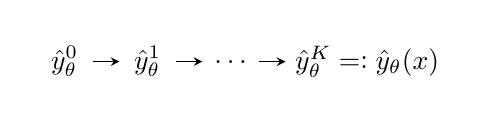
\begin{tikzpicture}
  \matrix (m) [
      matrix of math nodes,row sep=2em,column sep=1em,
      minimum width=2em,nodes={anchor=center}
  ] {
    \hat y^{0}_\theta & \hat y_\theta^{1} &
    \ldots & \hat y_\theta^{K}\eqdef \hat y_\theta(x) \\
  };
  \path[-stealth]
    (m-1-1) edge node {} (m-1-2)
    (m-1-2) edge node {} (m-1-3)
    (m-1-3) edge node {} (m-1-4);
\end{tikzpicture}
\end{center}
\vspace{-3mm}

One of the most common semi-amortized model is to
parameterize and integrate an optimization procedure
used to solve \cref{eq:opt} into the model $\hat y_\theta$,
such as gradient descent \citep{andrychowicz2016learning,finn2017model,kim2018semi}.
We emphasize that this optimization procedure is
an internal part of the amortization model $\hat y_\theta$,
often referred to as the \emph{inner-level} optimization
problem in the bi-level setting that arises for learning.

\textbf{Examples.}
We now instantiate a canonical semi-amortized model based
gradient descent that learns the initialization as in
model-agnostic meta-learning (MAML) by \citet{finn2017model},
structured prediction energy networks (SPENs) by \citet{belanger2017end},
and semi-amortized variational auto-encoders (SAVAEs) by \citet{kim2018semi}.
The initial iterate $\hat y^{0}_\theta(x)\defeq \theta$
is parameterized by $\theta\in\gX$ for all contexts.
We then use the knowledge of the objective $f(y;x)$
for a given context $x$ and iteratively update
\begin{equation}
  \hat y^{t}_\theta \defeq \hat y^{t-1}_\theta - \alpha \nabla_y f(\hat y^{t-1}_\theta; x) \qquad t\in\{1\ldots,K\}
  \label{eq:gd}
\end{equation}
for $K$ steps with a \emph{learning rate} $\alpha\in\R_+$
and set the model's output to be
$\hat y_\theta\defeq \hat y^{K}$.

Semi-amortized models over the domain can go significantly beyond
gradient-based models and in theory, any algorithm to solve
the original optimization problem in \cref{eq:opt}
can be integrated into the model.
We will further discuss the learning of semi-amortized
models by unrolling in \cref{sec:unrolled} and will
then later see many other instantiations of it:
\begin{itemize}
\item \Cref{sec:apps:lista} discusses how
\citet{gregor2010learning} integrate ISTA iterates
\citep{daubechies2004iterative,beck2009fast}
into a semi-amortized model.
\item \Cref{sec:apps:neural-fp} discusses models that integrate
fixed-point computations into semi-amortized models.
\citet{venkataraman2021neural} amortize convex cone programs by
differentiating through the splitting cone solver \citep{o2016conic}
and \citet{bai2022neural} amortize
deep equilibrium models \citep{bai2019deep,bai2020multiscale}.
\item \Cref{sec:apps:qprl} discusses RLQP by \citet{ichnowski2021accelerating}
  that uses the OSQP solver \citep{stellato2018osqp} inside
  of a semi-amortized model.
\end{itemize}

\subsubsection{Semi-amortized models over a latent space $\gZ$}
\label{sec:semi-latent}
\begin{center}
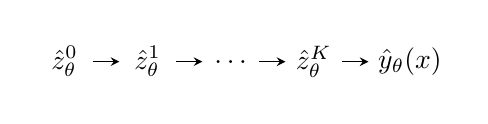
\begin{tikzpicture}
  \matrix (m) [
      matrix of math nodes,row sep=2em,column sep=1em,
      minimum width=2em,nodes={anchor=center}
  ] {
    \hat z^{0}_\theta & \hat z_\theta^{1} &
    \ldots & \hat z_\theta^{K} & \hat y_\theta(x) \\};
  \path[-stealth]
    (m-1-1) edge node {} (m-1-2)
    (m-1-2) edge node {} (m-1-3)
    (m-1-3) edge node {} (m-1-4)
    (m-1-4) edge node {} (m-1-5);
\end{tikzpicture}
\end{center}
\vspace{-3mm}

In addition to only updating iterates over the domain $\gY$,
a natural generalization is to introduce a latent space $\gZ$
that is iteratively optimized over \emph{inside} of
the amortization model.
This is usually done to give the semi-amortized model
more capacity to learn about the structure of the optimization
problems that are being solved.

\textbf{Examples.}
The iterative gradient updates in \cref{eq:gd}
can be replaced with a learned update function as in
\citet{ravi2016optimization,li2016learning,li2017learning}.
These model the past sequence of iterates and learn how
to best-predict the next iterate so that the overall
sequence is optimal.
This can be done with a recurrent cell $g$ such
as an LSTM \citep{hochreiter1997long} or GRU \citep{cho2014learning}
and leads to updates of the form
\begin{equation}
  z^t_\theta, \hat y^{t}_\theta \defeq g_\theta(z^{t-1}_\theta, x^{t-1}_\theta, \nabla_y f(\hat y^{t-1}_\theta; x)) \qquad t\in\{1\ldots,K\}
  \label{eq:rec}
\end{equation}
where each call to the recurrent cell $g$
takes a hidden state $z$ along with an iterate and
the derivative of the objective.
This endows $g$ with the capacity to learn significant
updates leveraging the problem structure that a
traditional optimization method would not be able
to make.
In theory, traditional update rules can also be
fallen back on as the gradient step in \cref{eq:gd}
is captured by removing the hidden state $z$ and
setting
\begin{equation}
  g(x, \nabla_y f(y; x))\defeq x-\alpha\nabla_y f(y; x).
  \label{eq:rec-grad-step}
\end{equation}

Latent semi-amortized models are a budding topic and can
excitingly learn many other latent representations
that go beyond iterative gradient updates in the original
space.
\citet{luo2018neural,amos2019dcem}
learn a \emph{latent domain} connected to the
original domain where the latent domain captures
hidden structures and redundancies present in
the original high-dimensional domain $\gY$.
\citet{luo2018neural} consider gradient updates
in the latent domain and \citet{amos2019dcem}
show that the cross-entropy method \citep{de2005tutorial}
can be made differentiable and learned as an alternative
to gradient updates.
\citet{amos2017input} unrolls and differentiates through
the bundle method \citep{smola2007bundle} in a convex setting
as an alternative to gradient steps.
The latent optimization could also be done over a learned parameter
space as in POPLIN \citep{wang2019exploring}, which \emph{lifts}
the domain of the optimization problem \cref{eq:opt}
from $\gY$ to the parameter space of a fully-amortized neural network.
This leverages the insight that the parameter space of
over-parameterized neural networks can induce easier
non-convex optimization problems than in the original
space, which is also studied in \citet{hoyer2019neural}.

\subsubsection{Semi-amortized models vs.~warm-starting and fine-tuning}
Semi-amortized models are conceptually similar to learning a fully-amortized model
to warm-start an existing optimization procedure that fine-tunes the solution.
The crucial difference is that semi-amortized learning often end-to-end learns
through the final prediction while warm-starting and fine-tuning only learns
the initial prediction and does not integrate the knowledge of the fine-tuning
procedure into the learning procedure.
Choosing between these is an active research topic and while we will
mostly focus on semi-amortized models, learning a fully-amortized
warm-starting model brings promising results to some fields too,
such as \citet{zhang2019safe,baker2019learning,chen2022large}.
In variational inference, \citet[Table 2]{kim2018semi} compare semi-amortized
models (SA-VAE) to warm-starting and fine-tuning (VAE+SVI) and demonstrate
that the end-to-end learning signal is helpful.
\citet{arbel2021amortized} further study fully-amortized warm-started
solvers that arise in bi-level optimization problems for
hyper-parameter optimization and use the theoretical framework from
singularly perturbed systems \citep{habets2010stabilite}
to analyze properties of the approximate solutions.

\subsubsection{On second-order derivatives of the objective}
\label{sec:second-derivatives}
Second-order derivatives of the objective often arise when optimizing
semi-amortized models and may be a computational bottleneck.
\citet{finn2017model,nichol2018first,lorraine2020optimizing}
propose alternatives to forming the full unrolled derivative,
and in this section we will take a closer look at where the
second-order terms come from and discuss alternatives.
\citet{finn2017model} observed these second-order terms and
the following derivation is similar to the ones that
\citet[\S5]{nichol2018first} and \citet{weng2018metalearning}
perform by composing the model with the loss, as we will expand on
in \cref{eq:grad-loss-grad}. We focus only on the
model derivatives.

\textbf{Starting with a single-step model.}
We first instantiate a single-step model
similar to \cref{eq:gd} that parameterizes the initial
iterate $\hat y^0_\theta(x)\defeq\theta$ and takes one gradient step:
\begin{equation}
  \hat y_\theta(x)\defeq \hat y^0_\theta(x) - \alpha \nabla_y f(\hat y^0_\theta(x); x)
  \label{eq:single-step}
\end{equation}
The Jacobian of $\hat y_\theta(x)$ with respect to the parameters is
\begin{equation}
  \D_\theta[\hat y_\theta(x)] = I-\alpha \nabla_y^2 f(y_\theta^0(x); x),
  \label{eq:second-derivatives-single-step}
\end{equation}
which requires the Hessian of the objective.
In \citet{finn2017model}, $\nabla_y^2 f$ is the Hessian of the
model's parameters on the training loss (!) and is
compute- and memory-expensive to obtain for large models.
Before discussing alternatives, we derive similar results for
a $K$-step model.

\textbf{Multi-step models.}
We extend \cref{eq:single-step} to the $K$-step setting with
\begin{equation}
\hat y_\theta^K(x)\defeq \hat y^{K-1}_\theta(x) - \alpha\nabla_y f(\hat y^{K-1}_\theta(x); x),
\end{equation}
where the base $\hat y_\theta^0(x)\defeq\theta$ as before.
Similar to \cref{eq:second-derivatives-single-step},
the derivative of a single step is
\begin{equation}
  \D_\theta[\hat y_\theta^K(x)] = \D_\theta[\hat y_\theta^{K-1}(x)]\left(I-\alpha\nabla_y^2 f(y_\theta^{K-1}(x); x)\right),
  \label{eq:second-derivatives-recurrent}
\end{equation}
and composing the derivatives down to $\hat y_\theta^0$ yields the product structure
\begin{equation}
  \D_\theta[\hat y_\theta^K(x)] = \prod_{k=0}^{K-1} \left( I-\alpha\nabla_y^2 f(y_\theta^k(x); x) \right),
  \label{eq:second-derivatives-k-steps}
\end{equation}
where we use $\D_\theta[\hat y_\theta^0(x)]=I$ at the base case.
Computing and storing \cref{eq:second-derivatives-k-steps} is
now $K$ times more challenging as it requires storing the Hessian
$\nabla_y^2 f$ at \emph{every} iteration of the model!

\textbf{Computationally cheaper alternatives.}
The first-order MAML baseline in \citet{finn2017model} suggests to
simply not use the second-order terms $\nabla_y^2 f$ here,
approximating the model derivative as the identity,
\ie $\D_\theta[\hat y_\theta^K(x)]\approx I$,
and relying on only information from the outer loss
to update the parameters.
They use the intuition from \citet{goodfellow2014explaining}
that neural networks are locally linear and therefore these
second-order terms of $f$ are not too important.
They show that this approximation works well in some cases,
such as MiniImagenet \citep{ravi2016optimization}.
The MAML$++$ extension by \citet{antoniou2018train} proposes to
use first-order MAML during the early phases of training, but
to later add back this second-order information.
\citet{nichol2018first} further analyze first-order approximations
to MAML and propose another approximation called Reptile that
also doesn't use this second-order information.
These higher-order terms also come up when unrolling in the
different bi-level optimization setting for hyper-parameter optimization,
and \citet[Table 1]{lorraine2020optimizing} gives
a particularly good overview of approximations to these.

\textbf{Parameterizing and learning the objective.}
While we mostly do not consider the setting when
the objective $f$ is also learned,
the second-order derivatives appearing in
\cref{eq:second-derivatives-k-steps}
also cause issues in when the objective is parameterized
and learned.
In addition to learning an initial iterate, \citet{belanger2017end}
the learn the objective $f$ representing an energy function.
They parameterize $f$ as a neural network and use softplus
activation functions rather than ReLUs to ensure the
objective's second-order derivatives exist.

\subsection{Models based on differentiable optimization}
As we will see in the next section, the model typically needs
to be (sub-)differentiable with respect to the parameters
to attain the derivative $\D_\theta[\hat y_\theta]$ necessary
to optimize the loss.
These derivatives are standard backprop when the model
is, for example, a full-amortized neural network, but
in the semi-amortized case, the model itself is often an
optimization process that needs to be differentiated through.
When the model updates are objective-based as in
\cref{eq:gd} and \cref{eq:rec}, the derivatives with respect
to $\theta$ through the sequence of gradient updates
in the domain can be attained by seeing the updates
as a sequence of computations that are differentiated through,
resulting in second-order derivatives.
When more general optimization methods are used for
the amortization model that may not have a closed-form
solution, the tools of differentiable optimization
\citep{domke2012generic,gould2016differentiating,amos2017optnet,amos2019differentiable,agrawal2019differentiable}
enable end-to-end learning.

\section{Learning the model's parameters $\theta$}
\label{sec:learning}

\begin{figure}[t]
  \centering
  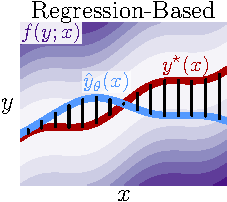
\includegraphics[width=0.32\textwidth]{fig/learning-reg.pdf}
  \hspace{10mm}
  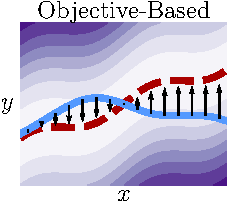
\includegraphics[width=0.32\textwidth]{fig/learning-obj.pdf}
  \caption{Overview of key learning methods for optimizing
    the parameters $\theta$ of the amortization model $\hat y_\theta$.
    1) Regression-based losses optimize a distance between
    the model's prediction $\hat y_\theta(x)$ and the
    ground-truth $y^\star(x)$, and 2) objective-based
    methods update $\hat y_\theta$ using
    local information of the objective $f$
    and \emph{without} access to the ground-truth
    solutions $y^\star$.
  }
  \label{fig:learning}
\end{figure}

Given an amortization model $\hat y_\theta$, the last remaining design choice
is how to learn the parameters $\theta$
so that the model best-solves \cref{eq:opt}.
Learning is often a \emph{bi-level} optimization problem
where the \emph{outer level} is the parameter
learning problem for a model $\hat y_\theta(x)$ that solves
the \emph{inner-level} optimization problem in \cref{eq:opt}
over the domain $\gY$.
While defining the best loss is application-specific,
most approaches can be roughly categorized as
1) matching a ground-truth solution (\cref{sec:learning:reg}),
or 2) minimizing the objective (\cref{sec:learning:grad,sec:learning:rl}),
which \cref{fig:learning} illustrates.
Optimizing the model parameters here can in theory be done
with most parameter learning methods that incorporate
zeroth-, first-, and higher-order information
about the loss being optimized, and in here we mostly focus
on methods where $\theta$ is learned with a
first-order gradient-based method
such as \citet{nesterov1983method,duchi2011adaptive,zeiler2012adadelta,kingma2014adam}.
We discuss key approaches of designing the loss
and optimizing the parameters with first-order methods
(\cref{sec:learning:reg,sec:learning:grad})
when differentiation is easy
or reinforcement learning (\cref{sec:learning:rl})
otherwise, \eg, in non-differentiable settings.

\subsection{Choosing the objective for learning}
\subsubsection{Regression-based learning}
\label{sec:learning:reg}
The first learning method we consider is to regress the
model's prediction $\hat y_\theta(x)$ onto a
ground-truth solution $y^\star(x)$.
These minimize some distance between the predictions
and ground-truth so that the expectation over
the context distribution $p(x)$ is minimal.
With a Euclidean distance, for example,
regression-based learning solves
\begin{equation}
  \argmin_\theta \gL_{\rm reg}(\hat y_\theta) \qquad
  \gL_{\rm reg}(\hat y_\theta) \defeq
  \E_{x \sim p(x)} \|y^\star(x) - \hat y_\theta(x) \|_2^2.
\label{eq:reg-loss}
\end{equation}
$\gL_{\rm reg}$ is typically optimized with an adaptive first-order
gradient-based method that is able to directly differentiate
the loss with respect to the model's parameters.

Regression-based learning works the best for distilling
known solutions into a faster model that can be deployed
at a much lower cost, but can otherwise start failing to work.
In control, regression-based amortization
methods are referred to as \emph{behavioral cloning}.
These methods work well when the ground-truth solutions
are unique and semi-tractable, but can fail otherwise,
\ie if there are many possible ground-truth
solutions for a context $x$ or if computing them
is too intractable.
After all, solving \cref{eq:opt} from scratch may be
computationally expensive and amortization methods
should improve the computation time.

\subsubsection{Objective-based learning}
\label{sec:learning:grad}

Instead of regressing onto the ground-truth solution,
\emph{objective-based} learning methods seek for
the model's prediction to be minimal under the objective $f$ with:
\begin{equation}
  \argmin_\theta \gL_{\rm obj}(\hat y_\theta) \qquad \gL_{\rm obj}(\hat y_\theta) \defeq \E_{x \sim p(x)} f(\hat y_\theta(x); x).
\label{eq:grad-loss}
\end{equation}
These methods use local information of the objective
to provide a descent direction for the model.
A first-order method optimizing \cref{eq:grad-loss} uses
updates based on the gradient
\begin{equation}
  \begin{aligned}
  \nabla_\theta \gL_{\rm obj}(\hat y_\theta) &= \nabla_\theta \left[ \E_{x\sim p(x)}f(\hat y_\theta(x); x)\right] \\
  &= \E_{x\sim p(x)} \D_\theta\left[ \hat y_\theta(x)\right]^\top
  \nabla_{y} \left[ f(\hat y_\theta(x); x) \right],
  \end{aligned}
  \label{eq:grad-loss-grad}
\end{equation}
where the last step is obtained by the chain rule.
This has the interpretation that the model's parameters $\theta$
are updated by combining the gradient information around the prediction
$\nabla_{x} \left[ f(\hat y_\theta(x); x) \right]$,
which we show in \cref{fig:learning},
with how $\theta$ impacts the model's predictions with the derivative
$\D_\theta\left[ \hat y_\theta(x)\right]$.
While we mostly focus on optimizing
\cref{eq:grad-loss-grad} with
first-order methods that explicitly differentiate
the objective, \cref{sec:learning:rl} discusses alternatives
to optimizing it with reinforcement learning and
zeroth-order methods.

Objective-based methods thrive when the gradient information
is informative and the objective and models are easily differentiable.
We will see that amortized variational inference methods and
actor-critic methods both make extensive use of
objective-based learning.

\begin{remark}
  A standard gradient-based optimizer for \cref{eq:opt} (without amortization)
  can be recovered from $\gL_{\rm obj}$ by setting the model to the identity
  of the parameters, \ie $\hat y_\theta(x)\defeq\theta$, and $p(x)$ to be a
  Dirac delta distribution.
  \label{remark:obj-loss}
\end{remark}

This can be seen by taking $\D_\theta[\hat y_\theta(x)]=I$
in \cref{eq:grad-loss-grad}, resulting in
$\nabla_\theta \gL_{\rm obj}(\hat y_\theta)=\nabla_y f(\hat y_\theta(x); x)$.
Thus optimizing $\theta$ of this parameter-identity model with gradient descent
is identical to solving \cref{eq:opt} with gradient descent.
\Cref{remark:obj-loss} shows a connection between a model trained with
gradients of an objective-based loss and a non-amortized gradient-based
solver for \cref{eq:opt}.
The gradient update that would originally have been applied to an
iterate $y\in\gY$ of the domain is now transferred into the
model's parameters that are shared across all problem instances.
This also leads us to the intuition that objective-based amortization
works best when a gradient-based optimizer is able to successfully
solve \cref{eq:opt} from scratch.

\subsubsection{Comparing the regression- and objective-based losses}
\begin{wrapfigure}{r}{1.8in}
% \vspace{-2mm}
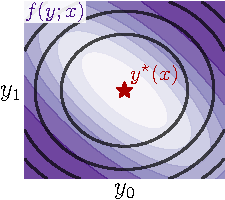
\includegraphics[width=\linewidth]{fig/loss-comp.pdf}\vspace{-3mm}
\caption{$\gL_{\rm reg}$ contours.}
% \vspace{-3mm}
\label{fig:reg-contours}
\end{wrapfigure}

Choosing between the regression- and objective-based losses
is challenging as they measure the solution quality in
different ways and have different convergence and
locality properties.
\citet{liu2022teaching} experimentally compare these
losses for learning to optimize with fully-amortized set-based models.
\Cref{fig:reg-contours} illustrates that the $\ell_2$-regression
loss (the black contours) ignores the objective
values (the purple contours) and thus gives the same loss
to solutions that result in significantly different
objective values.
This could be potentially addressed by normalizing or
re-weighting the dimensions for regression to be more aware
of the curvature of the objective, but this is often not done.
The following summarizes some other advantages ($+$) and
disadvantages ($-$):
\vspace{2mm}

\noindent
\begin{minipage}[t]{0.5\textwidth}
\noindent\textbf{Regression-based losses $\gL_{\rm reg}$}
\begin{itemize}[leftmargin=*,noitemsep]
\con Does not consider $f(y; x)$
\pro Uses global information with $y^\star(x)$
\con Expensive to compute $y^\star(x)$
\pro Does not compute $\nabla_y f(y; x)$
\con Hard to learn non-unique $y^\star(x)$
\end{itemize}
\end{minipage}
\begin{minipage}[t]{0.5\textwidth}
\textbf{Objective-based losses $\gL_{\rm obj}$}
\begin{itemize}[leftmargin=*,noitemsep]
\pro Uses objective information of $f(y; x)$
\con Can get stuck in local optima of $f(y; x)$
\pro Faster, does not require $y^\star(x)$
\con Often requires computing $\nabla_y f(y; x)$
\pro Easily learns non-unique $y^\star(x)$
\end{itemize}
\end{minipage}

\subsection{Learning iterative semi-amortized models}
\label{sec:learning:iter}

Fully-amortized or semi-amortized models can be learned
with the regression- and objective-based losses.
Here we discuss how the loss can be further opened up
and crafted to learn iterative semi-amortized methods.
For example, if the model produces intermediate predictions
$\hat y_\theta^i$ in every iteration $i$, instead of
optimizing the loss of just the final prediction,
\ie $\gL(\hat y_\theta^K)$, we can consider more generally
variants of the losses that we will denote as
$\gL^\Sigma$ that consider the impact of every iteration
of the model's prediction
\begin{equation}
  \argmin_\theta \gL^\Sigma(\hat y_\theta) \qquad \gL^\Sigma(\hat y_\theta) \defeq \sum_{i=0}^K w_i \gL(\hat y_\theta^i),
\label{eq:iter-loss}
\end{equation}
where $w_i\in\R_+$ are weights in every iteration $i$
that give a design choice of how important
it is for the earlier iterations to produce reasonable
solutions.
For example, setting $w_i=1$ encourages every iterate
to be low.

Learning iterative semi-amortized methods also has connections to
sequence learning models that arise in, \eg text, audio,
and language processing.
Given the context $x$, an iterative semi-amortized model
seeks to produce a sequence of predictions that ultimately
result in the intermediate and final predictions,
which can be analogous to a language model predicting
future text given the previous text as context.
We next discuss concepts that arise when computing the derivatives
of a loss with respect to the model's parameters.

\subsubsection{Unrolled optimization and backpropagation through time}
\label{sec:unrolled}
\begin{center}
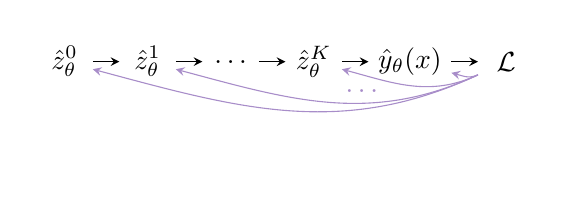
\begin{tikzpicture}
  \matrix (m) [
      matrix of math nodes,row sep=2em,column sep=1em,
      minimum width=2em,nodes={anchor=center}
  ] {
    \hat z^{0}_\theta & \hat z_\theta^{1} &
    \ldots & \hat z_\theta^{K} & \hat y_\theta(x) & \gL \\
    \; & \; & \; & \; & \; & \; \\};
  \node at (1.,0.1) () {\color{linkcolor}\ldots};
  \path[-stealth]
    (m-1-1) edge node {} (m-1-2)
    (m-1-2) edge node {} (m-1-3)
    (m-1-3) edge node {} (m-1-4)
    (m-1-4) edge node {} (m-1-5)
    (m-1-5) edge node {} (m-1-6)
    (m-1-6) edge[draw=linkcolor,out=-155,in=-15] node[below] {} (m-1-5)
    (m-1-6) edge[draw=linkcolor,out=-155,in=-15] node {} (m-1-4)
    (m-1-6) edge[draw=linkcolor,out=-155,in=-15] node {} (m-1-2)
    (m-1-6) edge[draw=linkcolor,out=-155,in=-15] node {} (m-1-1)
    ;
\end{tikzpicture}
\end{center}
\vspace{-10mm}

The parameterization of \emph{every} iterate $z_\theta^i$ can
influence the final prediction $\hat y_\theta$ and thus
losses on top of $\hat y_\theta$ need to consider the
entire chain of computations.
Differentiating through an iterative procedure such
as this is referred to as \emph{backpropagation through time}
in sequence models and \emph{unrolled optimization}
\citep{pearlmutter2008reverse,zhang2010multi,maclaurin2015gradient,belanger2016structured,metz2016unrolled,finn2017model,han2017alternating,belanger2017end,belanger2017deep,foerster2017learning,bhardwaj2020differentiable,monga2021algorithm}
when the iterates are solving an optimization problem
as the model computation is iterative and computing
$\D_\theta[\hat y_\theta(x)]$
requires saving and differentiating the ``unrolled''
intermediate iterations, as we saw in \cref{sec:second-derivatives}.
The terminology ``unrolling'' here emphasizes that the
iterative computation produces a compute graph of operations
and is likely inspired from
\emph{loop unrolling} in compiler optimization
\citep{aho1986compilers,davidson1995aggressive} where
loop operations are inlined for efficiency and written
as a single chain of repeated operations rather
than an iterative computation of a single operation.

Even though $\D_\theta \hat y_\theta$ is well-defined,
in practice it can be
instable because of exploding gradients,
and inefficient for compute and memory resources because
every iterate needs to be stored,
as we saw in \cref{sec:second-derivatives}.
This is why most methods using unrolled optimization for learning
often only unroll through \emph{tens} of iterations
\citep{metz2016unrolled,belanger2017end,foerster2017learning,finn2017model}
while solving the problems from scratch typically
require \emph{millions} (!) of iterations.
This causes the predictions to be extremely inaccurate solutions
to the optimization process and has sparked the research directions
that we next turn to that seek to make unrolled optimization
more tractable.

\subsubsection{Truncated backpropagation through time and biased gradients}
\begin{center}
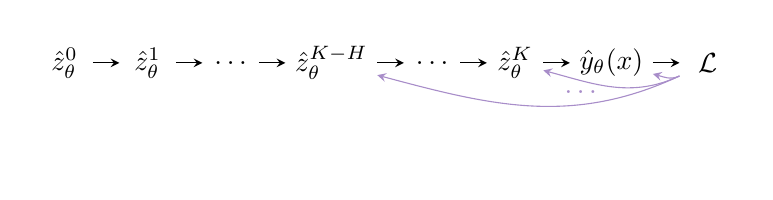
\begin{tikzpicture}
  \matrix (m) [
      matrix of math nodes,row sep=2em,column sep=1em,
      minimum width=2em,nodes={anchor=center}
  ] {
    \hat z^{0}_\theta & \hat z_\theta^{1} &
    \ldots & \hat z_\theta^{K-H} & \ldots &
    \hat z_\theta^{K} & \hat y_\theta(x) & \gL \\
    \; & \; & \; & \; & \; & \; \\};
  \node at (2.5,0.1) () {\color{linkcolor}\ldots};
  \path[-stealth]
    (m-1-1) edge node {} (m-1-2)
    (m-1-2) edge node {} (m-1-3)
    (m-1-3) edge node {} (m-1-4)
    (m-1-4) edge node {} (m-1-5)
    (m-1-5) edge node {} (m-1-6)
    (m-1-6) edge node {} (m-1-7)
    (m-1-7) edge node {} (m-1-8)
    (m-1-8) edge[draw=linkcolor,out=-155,in=-15] node[below] {} (m-1-7)
    (m-1-8) edge[draw=linkcolor,out=-155,in=-15] node {} (m-1-6)
    (m-1-8) edge[draw=linkcolor,out=-155,in=-15] node {} (m-1-4)
    ;
\end{tikzpicture}
\end{center}
\vspace{-10mm}

\emph{Truncated backpropagation through time (TBPTT)}
\citep{werbos1990backpropagation,jaeger2002tutorial}
is a crucial idea that has enabled the
training of sequence models over long sequences.
TBPTT's idea is that not every iteration needs to be
differentiated through and that the derivative
can be computed using smaller subsequences from
the full sequence of model predictions by
truncating the history of iterates.
For example, the derivative of a model running
for $K$ iterations with a truncation length of $H$
can be approximated by considering the
influence of the last $H$ iterates
$\left\{z_\theta^{i}\right\}_{i=K-H}^H$ on the loss $\gL$.

Truncation significantly helps improve the computational
and memory efficiency of unrolled optimization procedure
but results in harmful \emph{biased gradients} as
these approximate derivatives do not contain
the full amount of information that the model used
to compute the prediction.
This is especially damaging in approaches
such as MAML \citep{finn2017model} that \emph{only}
parameterize the first iterate and is why MAML-based
approaches often don't use TBPTT.
\citet{tallec2017unbiasing,wu2018understanding,liao2018reviving,shaban2019truncated,vicol2021unbiased}
seek to further theoretically understand the properties
of TBPTT, including the bias of the estimator
and how to unbias it.

In addition to truncating the iterations, other approaches
attempt to improve the efficiency of learning through
unrolled iterations with other approximations
that retain the influence of the entire sequence
of predictions on the loss
\citep{finn2017model,nichol2018first,lorraine2020optimizing}
we will further discuss in
\cref{sec:second-derivatives}.

\subsubsection{Semi-amortized learning with shrinkage and implicit differentiation}
\begin{wrapfigure}{r}{2.1in}
% \vspace{-2mm}
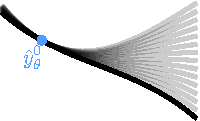
\includegraphics[width=\linewidth]{fig/imaml.pdf}
\captionsetup{font={small}}
\caption{\Cref{eq:iMAML} with varying $\lambda$.}
\label{fig:imaml}
\vspace{-3mm}
\end{wrapfigure}

A huge issue arising in semi-amortized models is that adapting
to long time horizons is computationally and memory inefficient
and even if it wasn't, causes exploding, vanishing, or
otherwise instable gradients.
An active direction of research seeks to solve these issues by
solving a smaller, local problem with the semi-amortized model,
such as in \citet{chen2019modular,rajeswaran2019meta}.
Implicit differentiation is an alternative to unrolling through
the iterations of a semi-amortized model in settings where the
model is able to successfully solve an optimization problem.
Here we briefly summarize \emph{Implicit MAML} (iMAML) by \citet{rajeswaran2019meta},
which notably brings this insight to MAML.
MAML methods usually only take a few gradient steps and
are usually not enough to globally solve \cref{eq:opt},
especially at the beginning of training.
\citet{rajeswaran2019meta} observe that adding a penalty
to the objective around the initial iterate
$\hat y^0_\theta$ makes it easy for the model to
\emph{globally} (!) solve the problem
\begin{equation}
  \label{eq:iMAML}
  \hat y_\theta(x) \in \argmin_y f(y; x) + \frac{\lambda}{2}\|y-\hat y^0_\theta\|_2^2,
\end{equation}
where the parameter $\lambda$ that encourages the
solution to stay close to some initial iterate.
In \cref{fig:imaml}, we visualize a function $f(y; x)$
in black and add penalties in grey with
$\lambda\in[0,12]$ and see that a global
minimum is difficult to find without adding a penalty
around the initial iterate.
This global solution can then be implicitly differentiated to obtain
a derivative of the loss with respect to the model's parameters
\emph{without} needing to unroll, as it requires
significantly less computational and memory resources.

\citet{huszar2019imaml} further analyzes and discuses iMAML.
They compare it to a Bayesian approach and observe that the insights
from iMAML can transfer from gradient-based meta-learning to
other amortized optimization settings.

\subsection{Parameter learning with zeroth-order methods
  and reinforcement learning}
\label{sec:learning:rl}

\begin{wrapfigure}{r}{2.0in}
\vspace{3mm}
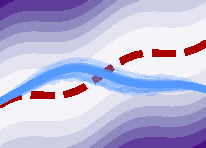
\includegraphics[width=\linewidth]{fig/learning-rl.pdf}
\caption{Perturbing $\hat y_\theta$.}
\vspace{-3mm}
\label{fig:perturbing}
\end{wrapfigure}

Computing the derivatives to learn $\hat y_\theta$ with a
first-order method may be impossible or instable.
These problems typically arise when learning components
of the model that are truly non-differentiable, or
when attempting to unroll a semi-amortized model for
a lot of steps.
In these settings, research has successfully explored
other optimizers that do \emph{not} need the gradient information.
These methods often consider settings that improve
an objective-based loss with small local perturbations
rather than differentiation.
\Cref{fig:perturbing} illustrates that most of these
methods can be interpreted as locally perturbing the
model's prediction and updating the parameters to
move towards the best perturbations.

\subsubsection{Reinforcement learning}
\citet{li2016learning,li2017learning,ichnowski2021accelerating} view their
semi-amortized models as a Markov decision process (MDP)
that they solve with reinforcement learning.
The MDP interpretation uses the insight
that the iterations $x^i$ are the actions,
the context and previous iterations or losses are typically the states,
the associated losses $\gL(x^i)$ are the rewards,
and $\hat y_\theta^i(x)$ is a (deterministic) policy,
and transitions given by updating the current iterate,
either with a quantity defined by the policy or by running
one or more iterations from an existing optimizer.
Once this viewpoint is taken, then the optimal amortized model
can be found by using standard reinforcement learning methods,
\eg \citet{li2016learning,li2017learning} uses Guided Policy Search \citep{levine2013guided}
and \citet{ichnowski2021accelerating} uses TD3 \citep{fujimoto2018td3}.
We use $\gL^{\rm RL}$ to indicate that a loss is optimized with reinforcement learning,
typically on the objective-based loss.

\subsubsection{Loss smoothing and optimization with zeroth-order methods}
\label{sec:smooth}

\begin{wrapfigure}{r}{2.1in}
\vspace{-2mm}
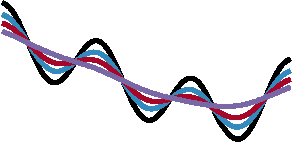
\includegraphics[width=\linewidth]{fig/smoothed-loss.pdf}
\captionsetup{font={small}}
\caption{\Cref{eq:smooth-loss} with varying $\sigma^2$.}
% \vspace{-1mm}
\label{fig:smooth-loss}
\end{wrapfigure}

\mbox{}\citet{metz2019understanding} observe that
objective-based losses can have a high-frequency
structure with many poor local minimum.
To overcome this, they use Gaussian smoothing:
\begin{equation}
  \gL^{\rm smooth}(\hat y_\theta)\defeq \E_{\epsilon\sim\gN(0,\sigma^2 I)}\left[\gL(\hat y_{\theta+\epsilon})\right],
  \label{eq:smooth-loss}
\end{equation}
where $\sigma^2$ is a fixed variance.
\Cref{fig:smooth-loss} illustrates a loss function $\gL$ in
black and shows smoothed versions in color.
They consider learning the loss with reparameterization
gradients and zeroth-order evolutionary methods.
\citet{merchant2021learn2hop} further
build upon this for learned optimization in
atomic structural optimization
and study 1)
clipping the values of the gradient estimator,
and 2) parameter optimization with genetic algorithms.

\begin{remark}
  TODO: Smoothing may change the global minimum.
\end{remark}

\textbf{Connection to smoothing in reinforcement learning.}
The Gaussian smoothing of the objective $\gL$ in \cref{eq:smooth-loss}
is conceptually similar to Gaussian smoothing of the
objective in reinforcement learning, \ie the $-Q$-value,
by a Gaussian policy that we will see in
\cref{eq:Q-opt-sto-exp} and further discuss
in \cref{sec:apps:ctrl}.
The policy's variance is typically controlled to match a
target entropy \citet{haarnoja2018soft} and the learning
typically starts with a high variance so the policy has a
broad view of the objective landscape and is then able to focus in
on a optimal region of the value distribution.
In contrast, \citet{metz2019understanding,merchant2021learn2hop}
do not turn the loss into a distribution and more directly
smooth the loss with a Gaussian with a fixed variance $\sigma^2$
that is not optimized over.

\section{Extensions of the amortization setting we consider here}
\label{sec:extensions}

I have intentionally scoped \cref{def:amor} to optimization problems
over \emph{deterministic, unconstrained, finite-dimensional, Euclidean}
domains $\gY$ where the context distribution $p(x)$
remains \emph{fixed} the
entire training time to provide a simple mental model that
allows us to focus on the core amortization principles
that consistently show up between applications.
Here, we cover extensions from this setting that may come up in practice.

\subsection{Extensions of the domain $\gY$}
\label{sec:extensions:domain}
\subsubsection{Deterministic $\rightarrow$ stochastic optimization}
\label{sec:extensions:sto}
A crucial extension is from optimization over deterministic vector
spaces $\gY$ to \emph{stochastic optimization}
where $\gY$ represents a space of distributions,
turning $y\in\gY$ from a vector in Euclidean space
into a distribution.
This comes up in \cref{sec:apps:ctrl} for control,
for example..

\textbf{Transforming parameterized stochastic problems
  back into deterministic ones.}
We will mostly focus on settings that optimize over
the parametric distributions.
We use this for the stochastic domains arising in amortized
variational inference in \cref{sec:apps:avi} and stochastic
control in \cref{sec:apps:ctrl}.
These settings optimize over a constrained parametric family
of distributions parameterized by some $\lambda$, for example
over a multivariate normal $\gN(\mu, \Sigma)$ parameterized
by $\lambda\defeq (\mu, \Sigma)$.
Here, problems can be transformed back to \cref{eq:opt} by
optimizing over the parameters with
\begin{equation}
  \lambda^\star(x) \in \argmin_{\lambda} f(\lambda; x),
  \label{eq:normal-opt}
\end{equation}
where $\lambda$ induces a distribution that the
objective $f$ may use.
When $\lambda$ is not an unconstrained real space, the
differentiable projections we will discuss in \cref{sec:constraints}
could be used to transform $\lambda$ back into this form for amortization.

\begin{wrapfigure}{r}{2.3in}
% \vspace{-2mm}
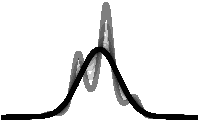
\includegraphics[width=\linewidth]{fig/maxent.pdf}
\captionsetup{font={small}}
\caption{Optimizing \cref{eq:maxent}.}
% \vspace{-2mm}
\end{wrapfigure}
\textbf{Optimizing over distributions and densities.}
More general stochastic optimization settings involve optimizing over
spaces representing distributions, such as the functional space
of all continuous densities.
Many standard probability distributions can be obtained and
characterized as the solution to a maximum entropy
optimization problem and is explored, \eg, in
\citet[Ch.~12]{cover2006elements},
\citet[p.~47]{guiasu1985principle}, and
\citet[\S6.2]{pennec2006intrinsic}.
For example, a Gaussian distribution $\gN(\mu, \Sigma)$
solves the following constrained maximum entropy
optimization problem over the space of continuous densities $\gP$:
\begin{equation}
  p^\star(\mu, \Sigma)\in \argmax_{p\in\gP} \HH_p[X]\; \subjectto\; \E_p[X] = \mu\; {\rm and}\; \Var_p[X] = \Sigma,
  \label{eq:maxent}
\end{equation}
where $\HH_p[X]\defeq -\int p(x)\log p(x){\rm d}x$ is the \emph{differential entropy}
and the constraints are on the mean $\E_p[X]$ and covariance $\Var_p[X]$.
\citet[Theorem~8.6.5 and Example~12.2.8]{cover2006elements} prove that the closed-form solution
of $p^\star$ is the Gaussian density.
This Gaussian setting therefore does not need amortization as the
closed-form solution is known and easily computed, but
more general optimization problems over densities do not necessarily
have closed-form solutions and could benefit from amortization.
While we do not study amortizing these problems, in some cases it may
be possible to again transform them back into deterministic optimization problems
over Euclidean space for amortization by approximating the density $g_\theta$
with an expressive family of densities parameterized by $\theta$.

\subsubsection{Unconstrained $\rightarrow$ constrained optimization}
\label{sec:constraints}
Amortized constrained optimization problems may naturally arise, for example
in the convex optimization settings we consider in \cref{sec:apps:convex}
and for optimization over the sphere we discuss in \cref{sec:apps:sphere}.
Constrained optimization problems for amortization can often be represented as
an extension of \cref{eq:opt} with
\begin{equation}
  y^\star(x) \in \argmin_{y\in\gC} f(y; x),
  \label{eq:opt-constrained}
\end{equation}
where the constraints $\gC$ may also depend on the context $x$
A budding research area studies how to more generally include
constraints into the formulation.
\citet{baker2019learning,dong2020smart,zamzam2020learning,pan2020deepopf}
learn to warm-start for optimal power flow.
\citet{misra2021learning} learn active sets for constrained optimization.
\citet{krivachy2020fast} solves constrained feasibility SDPs
with a fully-amortized neural network model using an
objective-based loss.
\citet{donti2021dc3} learns a fully-amortized model and optimizes an
objective-based loss with additional completion and correction terms
to ensure the prediction satisfies the constraints of the original problem.

\textbf{Differentiable projections.}
When the constraints are relatively simple, a differentiable projection
can transform a constrained optimization problem into an unconstrained one,
\eg, in reinforcement learning constrained action spaces can be transformed
from the box $[-1,1]^n$ to the reals $\R^n$ by using
the $\tanh$ to project from $\R^n$ to $[-1,1]^n$.
\Cref{sec:apps:sphere} also uses a differentiable projection from $\R^n$
onto the sphere $\gS^{n-1}$.
We define these as: \\

\noindent
\begin{minipage}{0.65\textwidth}
\begin{definition}
  A \emph{projection} from $\R^n$ onto a set $\gC\subseteq \R^n$ is
  \begin{equation}
    \pi_\gC: \R^n\rightarrow \gC \qquad \pi_\gC(x) \in \argmin_{y\in\gC} D(x, y) + \Omega(y),
    \label{eq:proj}
  \end{equation}
  where $D: \R^n\times\R^n\rightarrow \R$ is a distance and $\Omega:\R^n\rightarrow \R$ is
  a regularizer that can ensure invertibility or help spread $\R^n$ more uniformly throughout $\gC$.
  A \emph{(sub)differentiable projection} has (sub)derivatives $\nabla_x \pi_\gC(x)$.
  We sometimes omit the dependence of $\pi$ on the choice of $D$, $\Omega$, and $\gC$
  when they are given by the surrounding context.
  \label{def:proj}
\end{definition}
\end{minipage}
\begin{minipage}{0.35\textwidth}
  \hspace{8mm}
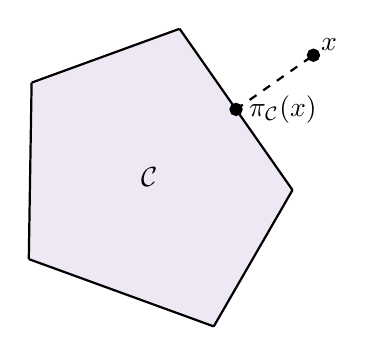
\begin{tikzpicture}[every path/.style={thick}]
  \path[fill=linkcolor!20] (0,0) coordinate(p1) -- ++(20:2) coordinate(p2) -- ++(-55:2.5)
    coordinate(p3) -- ++(-120:2.) coordinate(p4) --  ++(160:2.5) coordinate(p5);
 \node at (barycentric cs:p1=1,p2=1,p3=1,p4=1,p5=1) {$\gC$};
 \foreach \X [count=\Y] in {2,...,6} {
   \ifnum\X=6
     \path (p\Y) -- (p1) coordinate[pos=0.](a\Y) coordinate[pos=1.](a1)
       coordinate[pos=0.5](m1);
     \draw (a\Y) -- (a1);
  \else
     \path (p\Y) -- (p\X) coordinate[pos=0.](a\Y) coordinate[pos=1.](a\X)
       coordinate[pos=0.5](m\X);
     \draw (a\Y) -- (a\X);
  \fi}
 \draw[dashed] (m3) -- ($ (m3)!1.2cm!90:(p3) $) node[pos=1.2]{$x$}; %node[pos=-.3]{$\pi_\gC(x)$};
 \filldraw[black] (m3) circle(2pt);
 \filldraw[black] ($ (m3)!1.2cm!90:(p3) $) circle(2pt);
 \node[xshift=1pt,anchor=west] at (m3) {$\pi_\gC(x)$};
\end{tikzpicture}
\end{minipage} \\

\textbf{Lack of idempotency.} In linear algebra, a projection is defined to
be \emph{idempotent}, \ie applying the projection twice gives the same result
so that $\pi\circ \pi=\pi$.
Unfortunately, projections as defined in \cref{def:proj},
such as Bregman projections, are \emph{not} idempotent in general
and often $\pi_\gC\circ \pi_\gC\neq \pi_\gC$
as the regularizer $\Omega$ may cause points that are already on $\gC$
to move to a different position on $\gC$.

\textbf{Differentiable projections for constrained amortization.}
These can be used to cast \Cref{eq:opt-constrained} as the unconstrained
problem \cref{eq:opt} by composing the objective with a projection
$f\circ \pi_\gC$.
(Sub)differentiable projections enable gradient-based learning through the projection
and is the most easily attainable when the projection has an explicit closed-form solution.
For intuition, we first interpret the ReLU, sigmoid, and softargmax as
differentiable projections that solve convex optimization problems
in the form of \cref{eq:proj}.
\citet[\S2.4.4]{amos2019differentiable} further discusses these
and proves them using the KKT conditions:
\begin{itemize}
\item The standard Euclidean projection onto the
  \emph{non-negative orthant} $\R^n_+$ is defined by
  \begin{equation}
    \pi(x) \in \argmin_y \;\; \frac{1}{2}\|x-y\|_2^2 \;\; \st \;\; y\geq 0,
    \label{eq:relu-proj}
  \end{equation}
  and has a closed-form solution given the
  \emph{ReLU}, \ie $\pi(x) \defeq \max\{0, x\}$.
\item The interior of the \emph{unit hypercube} $[0,1]^n$ can
  be projected onto with the entropy-regularized
  optimization problem
  \begin{equation}
    \pi(x) \in \argmin_{0<y<1} \;\; -x^\top y -H_b(y),
    \label{eq:sigmoid-proj}
  \end{equation}
  where
  \begin{equation}
  H_b(y) = \defeq \left(\sum_i y_i\log y_i + (1-y_i)\log (1-y_i)\right)
  \end{equation}
  is the
  binary entropy function.
  \Cref{eq:sigmoid-proj} has a closed-form solution given by
  the \emph{sigmoid} or \emph{logistic} function,
  \ie $\pi(x) \defeq (1+e^{-x})^{-1}$.
\item The interior of the $(n-1)$-\emph{simplex} defined by
  \begin{equation}
    \Delta_{n-1}\defeq\{p\in\R^n\; \vert\; 1^\top p = 1 \; \; {\rm and} \;\; p \geq 0 \}
    \label{eq:simplex}
  \end{equation}
  can be projected onto with the entropy-regularized
  optimization problem
  \begin{equation}
    \pi(x) \in \argmin_{0<y<1} \;\; -x^\top y - H(y) \;\; \st\;\; 1^\top y = 1
    \label{eq:simplex-proj}
  \end{equation}
  where $H(y) \defeq -\sum_i y_i \log y_i$ is the entropy function.
  \Cref{eq:simplex-proj} has a closed-form solution given by
  the \emph{softargmax}, \ie $\pi(x)_j = e^{x_j} / \sum_i e^{x_i}$,
  which is historically referred to as the \emph{softmax}.
\end{itemize}

Going beyond these, we next cover differentiable projections onto
\emph{convex cones}, noting that they can also be softened or regularized
to help with continuity when composed with learning and
amortization methods.
\citet{ali2017semismooth,busseti2019solution} discuss
differentiating the standard Euclidean projections
onto these, including:
\begin{itemize}
\item
  \begin{minipage}[t]{0.65\textwidth}
  The \emph{second-order, Lorentz, or ice cream cone}
  defined by
  $\gK_{\rm soc}\defeq\{(x,y)\in\R^{m-1}\times\R : \|x\|_2\leq y\}$.
  The standard Euclidean projection is given in closed form as
  \begin{equation}
    \pi(x, y) \defeq
    \begin{cases}
      0 & \|x\|_2 \leq -y \\
      (x,y) & \|x\|_2 \leq y \\
      \frac{1}{2} (1 + \frac{y}{\|x\|_2}) (x, \|x\|_2) & \textrm{otherwise}.
    \end{cases}
  \end{equation}
  and can be explicitly differentiated.
  \end{minipage}
  \hspace{8mm}
  \begin{minipage}[t]{0.2\textwidth}
  \vspace{-2mm}
  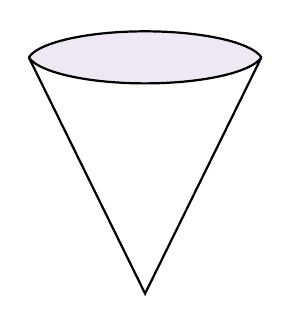
\begin{tikzpicture}[every path/.style={thick}]
    \path[fill=linkcolor!20]
      (0,0) arc (-170:-10:1.5cm and 0.4cm)coordinate[pos=0]
      -- (0,0) arc (170:10:1.5cm and 0.4cm)coordinate;
    \draw (0,0) arc (-170:-10:1.5cm and 0.4cm)coordinate[pos=0] (a);
    \draw (0,0) arc (170:10:1.5cm and 0.4cm)coordinate (b);
    \draw (a) -- ([yshift=-3cm]$(a)!0.5!(b)$) -- (b);
  \end{tikzpicture}
  \end{minipage}
\item The \emph{positive semidefinite cone} $\gS^m_+$ of the
  space of $m\times m$ positive semidefinite matrices.
  The Euclidean projection is obtained in closed-form
  by projecting the eigenvalues to be non-negative with
  $\pi(X)\defeq\sum_i\max\{\lambda_i, 0\}q_iq_i^\top$,
  where the eigenvalue decomposition of $X$ is given by
  $X=\sum_i\lambda_iq_iq_i^\top$.
  The derivative can be computed by differentiating
  through the eigenvalue decomposition and projection
  of the eigenvalues.
\item The \emph{exponential cone} is given by
  \begin{equation}
  \gK_{\rm exp}=\{(x,y,z) : x\in\R, y>0, z\geq y\exp(x/y)\}\cup
  \{(x,0,z): x\leq0, z\geq 0\}.
  \label{eq:exp-cone}
  \end{equation}
  The standard Euclidean projection onto this does
  \emph{not} have a known closed-form solution
  but can be computed using a Newton method
  as discussed in
  \citet[\S6.3.4]{parikh2014proximal}.
  \citet{ali2017semismooth} differentiate through
  this projection using implicit differentiation
  of the KKT system.
\end{itemize}

\noindent Other uses of projections in machine learning include:
\begin{itemize}
\item \citet{adams2011ranking,santa2017deeppermnet,mena2018learning}
  project onto the \emph{Birkhoff polytope} of
  \emph{doubly stochastic} matrices with row and
  column sums of 1, \ie
  \begin{equation}
    \label{eq:birkhoff}
    \gB_m\defeq \{X\in\R^{m\times m}: X1=X^\top1=1\}.
  \end{equation}
\item \citet{amos2019limited} project onto the capped
  simplex for a differentiable top-$k$ layer.
\item \citet{blondel2019structured} perform structure
  prediction and learning methods building on Fenchel-Young losses
  \citep{blondel2020learning} and use projections onto the
  simplex, unit cube, knapsack polytope, Birkhoff polytope,
  permutahedron, and order simplex.
\end{itemize}

In many of these, the projections have explicit closed-form
solutions that make it easy to compute and differentiate
through the projections for learning.
When a closed-form solution to the projection is not available to
the project, but the projection can be numerically computed,
projections can often still be differentiated through using
implicit differentiation.

\subsubsection{Euclidean $\rightarrow$ non-Euclidean optimization}
Manifold optimization \citep{absil2009optimization,hu2019brief}
over non-Euclidean spaces is a thriving topic in optimization
as these problems arise frequently over complex geometries in nature.
This area of research has studied acceleration methods,
\citep{duruisseaux2022accelerated}, less exploration
has been done on amortized optimization.
\Cref{sec:apps:sphere} discusses amortizing a simple
constrained spherical optimization problem that we are able
to transform into an unconstrained Euclidean optimization
problem by using projections from ambient Euclidean space.
When this is not possible, a budding area of research investigates
more directly including the manifold structure into the
amortization process. \citet{gao2020learning} amortize optimization
problems over SPD spaces.

\subsection{Extensions of the model $\hat y_\theta$}
Finding the best model for an amortized optimization setup
is an active research topic in many areas.
While we will mostly scope this tutorial to differentiable
parametric models that are end-to-end learned,
variations and extensions can be considered.

\subsubsection{Symbolic models: Uncovering human-interpretable update rules}
One of the largest issues in the models we consider
is that they are uninterpretable and it is often impossible
for us as humans to learn any new insights about the optimization
problems we are modeling, \eg how to better-solve them.
Symbolic models are one potential answer to this that attempt
to search over a symbolic space that is much closer to the
operations that humans would use to implement update rules for
an optimization solver.
Early studies of these methods include
\citet{bengio1994use,runarsson2000evolution}.
\citet{bello2017neural} significantly advances this direction
by posing the learned optimizer as a reinforcement learning problem
where the actions produce the operations underlying the update rules.
They show how existing methods can be symbolically implemented
using this formulation, and learn better update rules for
classification and machine translation tasks.
Symbolic methods are further studied and scaled in
\citet{real2020automl,zheng2022symbolic}.

This direction of work challenges the best accelerated and adaptive
gradient-based optimizers that are used for machine learning.
Nesterov acceleration \citep{nesterov1983method} has a provably
optimal convergence rate among first-order methods for solving
convex optimization problems, but unfortunately breaks down
in the non-convex setting.
This has led to a stream of variations of acceleration methods
for non-convex problems that come up in machine learning,
such as \citet{duchi2011adaptive,zeiler2012adadelta,kingma2014adam},
that typically add components that adapt the update rules to
how much the objective is moving in each dimension.
None of these algorithms are theoretically or provably the
best in non-convex settings, and is often empirically validated
depending on the domain.
Using amortized optimization with a symbolic model to search
the design space of optimizers can result is significantly
better optimizers and insights into the optimization problems
being solved, especially when this is done on new classes
of problems beyond the parameter learning problems typically
considered in machine learning settings.

\subsection{Uncertainty-aware and Bayesian optimization}
An active research direction combines \emph{uncertainty} estimation
and amortized optimization:

\textbf{Amortization for Bayesian optimization.}
\citet{chen2017learning} propose to use an RNN-based
  amortization in Bayesian optimization settings that
  predict the optimal solution to commonly used
  acquisition functions such as the expected improvement
  and observed improvement.
  This is powerful as optimizing the acquisition function
  is often a computational bottleneck.
\citet{swersky2020amortized} consider amortized
  Bayesian optimization in discrete spaces and show
  applications to protein sequence design.
\citet{ravi2018amortized} propose amortized
  Bayesian meta-learning for meta-learning with uncertainty
  estimation over the posterior and show applications to
  contextual bandits and few-shot learning.

\textbf{Bayesian methods for amortization.}
\citet{you2022bayesian} investigate \emph{optimizer uncertainty}
or \emph{Bayesian learning to optimize}.
This setting explores the uncertainty that an optimizer,
\eg the amortization model, is the best optimizer for
the problem.


\subsection{Settings where $p(x)$ changes and can be end-to-end learned}
We will mostly assume that $p(x)$ is fixed and remains
the same through the entire training process to allow us
to scope to the amortization aspects in all of the settings.
However, in some settings $p(x)$ may shift over time, which
could come from 1) the data generating process naturally
changing, or 2) a \emph{higher-level} learning process
also influencing $p(x)$.

Higher-level learning processes can use end-to-end learning
to update a context distribution parameterized by
$\varphi$, which we write as $p(x; \varphi)$.
This is done in, for example, variational inference
and deep equilibrium models, and involves optimizing
a higher-level loss $\ell$ defined on the \emph{solutions},
which could take the form of the bi-level problem
\begin{equation}
  \argmin_{\varphi} \E_{x\sim p(x; \varphi)} \ell(y^\star(x); x)\;
  \subjectto\; y^\star(x)\in\argmin_y f(y; x)
\label{eq:learn-context}
\end{equation}
where $y^\star(x)$ can be replaced with an approximation
by a learned amortization model $\hat y_\theta \approx y^\star$.
The parameters $\varphi$ in \cref{eq:learn-context} can
often by end-to-end learned \emph{through the solution} of
\cref{eq:opt} to update the influence that $p(x; \varphi)$
has on the solutions.
We next turn to methods that show how to differentiate
through the value $f(y^\star(x); x)$ and solution
$y^\star(x)$ to enable gradient-based learning of
$\varphi$ in \cref{eq:learn-context}.

\subsubsection{End-to-end learning $p(x; \varphi)$ by differentiating
  the value $f(y^\star(x); x)$}
Methods can end-to-end learn through the \emph{optimal value}
$f(y^\star(x); x)$ to update other parameters that show up
in the context.
For example, variational autoencoders differentiate through
the value, \ie the best approximation to the ELBO,
to optimize their density model.
The theory of \emph{why} this works is rooted in the
optimization community's studies of
\emph{envelope theorems}
that describe settings where the minimum value
can be differentiated by just differentiating
the objective.
\emph{Danskin's envelope theorem} \citep{danskin1966theory}
in convex settings is one of the earliest and has been
extended into more general settings, \eg, in
\citep[Prop. A.22]{bertsekas1971control}
and \cite{carter2001foundations,milgrom2002envelope,bonnans2013perturbation}.
In the unconstrained and non-convex \cref{eq:opt},
the envelope theorem gives
\begin{equation}
  \nabla_x \min_y f(y; \bar x) = \nabla_x f(y^\star(\bar x); \bar x)
  \label{eq:envelope}
\end{equation}
at a point $\bar x$ under mild assumptions, showing
that differentiating through the $\min$ operation is equivalent to differentiating
through just the objective at the optimal solution $y^\star(x)$.

\subsubsection{End-to-end learning $p(x)$ by differentiating the solution $y^\star(x)$}
In addition to differentiating through the value, the solution
$y^\star(x)$ can be implicitly differentiated.
We will refer to the derivative $\D_x y^\star(x)$
as the \emph{adjoint derivative}, and it is often used for
end-to-end learning
\citep{domke2012generic,gould2016differentiating,amos2017optnet,barratt2018differentiability,amos2019differentiable,agrawal2019differentiable,bai2019deep,bai2020multiscale}
and perturbation and sensitivity analysis
\citep{bank1982non,fiacco1990sensitivity,shapiro2003sensitivity,klatte2006nonsmooth,bonnans2013perturbation,still2018lectures,fiacco2020mathematical}.

Computing the adjoint derivative $\D_x y^\star(x)$ is more involved
than the value derivative using the envelope theorem
in \cref{eq:envelope} as more components of $y^\star(x)$
can change as $x$ moves infinitesimally.
An explicit closed-form solution to $y^\star(x)$ is
not available in most cases, which means that standard
methods for explicitly computing the derivative through
this computation may not work well or may break down.
For example, an optimizer to compute $y^\star(x)$ may be
explicitly unrolled through, but as we have seen in the
other settings, this may be instable and tracking all
of the iterations is extremely memory- and
compute-intensive.
The adjoint derivative is typically computed with implicit
differentiation by seeing $y^\star(x)$ as an \emph{implicit}
function of $x$.
This uses the implicit function theorem,
which is originally from \citet{dini1878analisi},
and is presented in \citet[Theorem 1B.1]{dontchev2009implicit} as:
\begin{theorem}[Dini's implicit function theorem]
  \label{thm:dini}
  Let the roots of $g(y; x)$ define an implicit
  mapping $Y^\star(x)$ given by $Y^\star(x)\defeq\{y \mid g(y;x)=0\}$,
  where $x\in\R^m$, $y\in\R^n$, and
  $g: \R^n\times\R^m\rightarrow\R^n$.
  Let $g$ be continuously differentiable in a neighborhood of $(\bar y, \bar x)$
  such that $g(\bar y; \bar x)=0$, and let the Jacobian of $g$
  with respect to $y$ at $(\bar y, \bar x)$,
  \ie $\D_y g(\bar y; \bar x)$, be non-singular.
  Then $Y^\star$ has a single-valued localization $y^\star$
  around $\bar x$ for $\bar y$ which is continuously differentiable
  in a neighborhood $Q$ of $\bar x$ with Jacobian satisfying
  \begin{equation}
    \D_x y^\star(\tilde x) = -\D_y^{-1} g(y^\star(\tilde x); \tilde x) \D_x g(y^\star(\tilde x); \tilde x)
    \qquad \mathrm{for\ every}\; \tilde x\in Q.
    \label{eq:implicit-derivative}
  \end{equation}
\end{theorem}

The adjoint derivative $D_x y^\star(x)$ can be computed
by seeing $y^\star$ as the roots of an implicit
function $g(y;x)$, which we need to select to
make the solution equivalent to the solution
of \cref{eq:opt}.
Typically $g(y;x)$ is an optimality system of
the optimization problem, \eg the KKT system
for constrained convex optimization problems.
For the unconstrained problem we consider here,
we can take the first-order optimality of
the objective $g(y;x) \defeq \nabla_y f(y; x)$
and apply \cref{thm:dini} to compute
$\D_x y^\star(x)$.

\begin{table*}[h]
  \caption{We tour the following applications of amortized optimization.}
  \vspace{3mm}
  % Copyright (c) Meta Platforms, Inc. and affiliates.
\hspace*{-8mm}
\resizebox{1.1\textwidth}{!}{
\begin{tabular}{ccccccc}
\S & Application & Objective $f$ & Domain $\gY$ & Context Space $\gX$ & Amortization model $\hat y_\theta$ & Loss $\gL$ \\ \toprule
\ref{sec:apps:avi} & VAE & $-\ELBO$ & variational posterior & data & full & $\gL_{\rm obj}$ \\
& SAVAE/IVAE & | & | & | & semi & | \\
\midrule
\ref{sec:apps:lista} & PSD & reconstruction & sparse code & data & full & $\gL_{\rm reg}$ \\
& LISTA & | & | & | & semi & | \\
\midrule
\ref{sec:apps:meta} & HyperNets & task loss & model parameters & tasks & full & $\gL_{\rm obj}$ \\
& LM & | & | & | & semi & $\gL^{\rm RL}_{\rm obj}$ \\
& MAML & | & | & | & | & $\gL_{\rm obj}$ \\
& Neural Potts & pseudo-likelihood & | & protein sequences & full & $\gL_{\rm obj}$ \\
\midrule
\ref{sec:apps:convex} & NeuralFP & FP residual & FP iterates & FP contexts & semi & $\gL_{\rm obj}^\Sigma$ \\
& HyperAA & | & | & | & | & $\gL_{\rm reg}^\Sigma$ \\
& NeuralSCS & CP residual & CP iterates & CP parameters & | & $\gL_{\rm obj}^\Sigma$ \\
& HyperDEQ & DEQ residual & DEQ iterates & DEQ parameters & | & $\gL_{\rm reg}^\Sigma$ \\
& NeuralNMF & NMF residual & factorizations & input matrices & | & $\gL_{\rm obj}^\Sigma$ \\
& RLQP & $R_{\rm RLQP}$ & QP iterates & QP parameters & | & $\gL^{\rm RL}_{\rm obj}$ \\
\midrule
\ref{sec:apps:ot} & AmorConj & $c$-transform obj & ${\rm supp}(\alpha)$ & ${\rm supp}(\beta)$ & full & $\gL_{\rm obj}$ \\
  & $\gA$-SW & max-sliced dist & slices $\Theta$ & mini-batches & | & $\gL_{\rm obj}$ \\
  & Meta OT & dual OT cost & optimal couplings & input measures & | & $\gL_{\rm obj}$ \\
\midrule
\ref{sec:apps:ctrl} & BC/IL & $-Q$-value & controls & state space & full & $\gL_{\rm reg}$ \\
& (D)DPG/TD3 & | & | & | & | & $\gL_{\rm obj}$ \\
& PILCO & | & | & | & | & $\gL_{\rm obj}$ \\
& POPLIN & | & | & | & full or semi & $\gL_{\rm reg}$ \\
& DCEM & | & | & | & semi & $\gL_{\rm reg}$ \\
& IAPO & | & | & | & | & $\gL_{\rm obj}$ \\
& SVG & $\D_\gQ$ or $-\gE_Q$ & control dists & | & full & $\gL_{\rm obj}$ \\
& SAC & | & | & | & | & $\gL_{\rm obj}$ \\
& GPS & | & | & | & | & $\gL_{\rm KL}$ \\
\midrule
\ref{sec:apps:sphere} & synthetic sphere & $c$-convex functions & $\gS^2\rightarrow \R^3$ & RCPM parameters & full & $\gL_{\rm obj}$ \\
\bottomrule
\end{tabular}}

%%% Local Variables:
%%% coding: utf-8
%%% mode: latex
%%% TeX-master: "amor"
%%% End:

  \label{tab:rw}
\end{table*}

\section{Review and tour of existing research that uses amortized optimization}
\label{sec:apps}
We now take a review and tour of the key applications
of amortized optimization to show some unifying ideas
that can be shared between all of these topics.
\Cref{tab:rw} summarizes the methods.
The subsections in here are meant to be standalone
and can be randomly accessed and read in any order.
I scope closely to providing the relevant context for
just the amortized optimization components and
under-emphasize the remaining context of each research area.

\textbf{Warning.}
Even though I try to provide the relevant background and notation to
present the amortized optimization components, each section is
meant to be a review rather than an introduction to
these research topics.
I defer further background to the original literature.

\subsection{Amortized variational inference and
  variational autoencoders}
\label{sec:apps:avi}
Key ideas in amortized optimization originated in the
variational inference (VI) community's interest in
approximating intractable densities and integrals
via optimization.
We focus on the relevant components of amortized
variational inference (AVI) used in machine learning
for the variational autoencoder (VAE) and
related generative models
\citep{kingma2013auto,rezende2014stochastic,mnih2014neural,rezende2015variational,higgins2016beta,doersch2016tutorial,kingma2019introduction}
and refer to references such as
\citet{jordan1999introduction,wainwright2008graphical,blei2017variational}
for a complete background in variational inference.
\citet{kim2020deep,marino2021learned} provide additional background
on the use of amortization and semi-amortization in these settings.
Historically, the use of an encoder network for amortized inference
is often traced back to the Helmholtz machine \citep{dayan1995helmholtz},
which uses a fully-amortized model but without a proper gradient estimator.

\subsubsection{The variational autoencoder (VAE) by \citet{kingma2013auto}}
A VAE models a density $p(x)$ over a high-dimensional space,
for example images, text, or videos, given samples $x\sim p(x)$.
They introduce a lower-dimensional latent space
with a known distribution $p(z)$, such as an isotropic Gaussian,
designed to capture hidden structure present
in $p(x)$.
Before defining the amortization model,
VAEs parameterize a likelihood model $p(x; \varphi)$ with $\varphi$.
Optimizing the log-likelihood
$\log p(x; \varphi)=\log\int_z p(x\mid z; \varphi)p(z)dz$
with this latent structure is typically intractable because
of the integral over the latent space.
Variational methods overcome this by introducing
a tractable lower-bound called the
\emph{evidence lower bound} ($\ELBO$) defined by
\begin{equation}
  \log p(x; \varphi)\geq \ELBO(\lambda; x, \varphi) \defeq \E_{q(z; \lambda)}[\log p(x\mid z; \varphi)] - \kl{q(z;\lambda)}{p(z)},
  \label{eq:elbo}
\end{equation}
where $q(z; \lambda)$ is a variational distribution
over the latent space parameterized by $\lambda$
and $p(z)$ is the prior.
Given a sample $x\sim p(x)$, we can find the \emph{best}
lower bound $\lambda^\star$ that satisfies
\begin{equation}
  \log p(x)\geq \ELBO(\lambda^\star; x, \varphi) \geq \ELBO(\lambda; x, \varphi)
  \label{eq:best-elbo}
\end{equation}
for all $\lambda$ by solving the optimization problem
\begin{equation}
  \lambda^\star \in \argmax_\lambda\; \ELBO(\lambda; x, \varphi).
  \label{eq:elbo-opt}
\end{equation}

Amortized VI (AVI) methods predict the solution to
\cref{eq:elbo-opt} while stochastic variational
methods \citep{hoffman2013stochastic} explicitly solve it.
AVI methods learn a model $\hat \lambda_\theta: \gX\rightarrow \Lambda$
with parameters $\theta$, which is usually a feedforward neural network,
to predict the maximum value of the $\ELBO$ by optimizing
the objective-based loss
\begin{equation}
  \argmax_\theta \E_{x\sim p(x)} \ELBO(\hat \lambda_\theta(x); x, \varphi)
  \label{eq:vae-amor}
\end{equation}
where the expectation is usually approximated with a
Monte Carlo estimate from the samples.

\textbf{Summary.} This standard AVI formulation is therefore an amortized optimization method
$\gA_{\rm VAE}\defeq (-\ELBO, \Lambda, \gX, p(x), \hat \lambda_\theta, \gL_{\rm obj})$
over the (negated) $\ELBO$ where the domain of the optimization
problem is the variational parameter space $\Lambda$,
the context space $\gX$ is the sample space for the
generative model,
the samples are given from $p(x)$,
$\hat\lambda_\theta: \gX\rightarrow\Lambda$ is the
\emph{fully-amortized} model optimized with the
gradient-based loss $\gL_{\rm obj}$ over $-\ELBO$.

\textbf{Extensions.}
Analyzing and extending the amortization components
has been a key development in AVI methods.
\citet{cremer2018inference} investigate suboptimality in
these models are categorize it as coming from an
\emph{amortization gap} where the amortized model for
\cref{eq:vae-amor} does not properly solve it,
or the \emph{approximation gap} where the variational
posterior is incapable of approximating the true distribution.
Semi-amortization plays a crucial role in addressing the
amortization gap and is explored in the
semi-amortized VAE (SAVAE) by \citet{kim2018semi}
and iterative VAE (IVAE) by \citet{marino2018iterative}.

\textbf{The full VAE loss.}
This section has left the parameterization
$\varphi$ of the model $p(x; \varphi)$
fixed to allow us to scope into the
amortized optimization component in isolation.
For completeness, the final step necessary to train
a VAE is to optimize the $\ELBO$ over the training
data of \emph{both} $p(x; \varphi)$ along with
the $\hat \lambda_\theta(x)$ with
\begin{equation}
  \argmax_{\varphi,\theta} \E_{x\sim p(x)} \ELBO(\hat \lambda_\theta(x); x, \varphi).
  \label{eq:vae-full}
\end{equation}

\subsection{Amortized sparse coding}
\label{sec:apps:lista}
Another early appearance of amortized optimization has been in
sparse coding \citep{kavukcuoglu2010fast,gregor2010learning}.
The connection to the broader amortized optimization and
learning to optimize work has also been made by,
\eg, \citet{chen2021learning}.
\emph{Sparse coding methods} seek to reconstruct an input
from a sparse linear combination of bases
\citep{olshausen1996emergence,chen2001atomic,donoho2003optimally}.
Given a \emph{dictionary} $W_d$ of the basis vectors
and an input $x\in\gX$, the \emph{sparse code} $y^\star$ is
typically recovered by solving the optimization problem
\begin{equation}
  y^\star(x) \in \argmin_y E(y; x) \qquad
  E(y; x)\defeq \frac{1}{2}\|x-W_dy\|_2^2 + \alpha\|y\|_1,
  \label{eq:sparse-coding}
\end{equation}
where $E$ is the regularized reconstruction energy
and $\alpha\in\R_+$ is a coefficient of the $\ell_1$ term.
\Cref{eq:sparse-coding} is traditionally solved
with the Iterative Shrinkage and Thresholding Algorithm (ISTA)
such as in \citet{daubechies2004iterative}.
Fast ISTA (FISTA) by \citet{beck2009fast} improves ISTA even more
by adding momentum term.
The core update of ISTA methods is
\begin{equation}
  y^{t+1}\defeq h_\beta\left(W_ex + Sy^t\right)
  \label{eq:ista}
\end{equation}
$W_e\defeq (1/L)W_d^\top$ is the \emph{filter} matrix,
$L$ is an \emph{upper bound on the largest eigenvalue} of $W_d^T W_d$,
$S\defeq I-W_eW_d$ is the \emph{mutual inhibition} matrix,
and
$h_\beta(v)\defeq\sign(v)\max\left\{0, |v|-\beta\right\}$
is the \emph{shrinkage function} with threshold $\beta$, usually
set to $\alpha/L$.
ISTA methods are remarkably fast ways of solving
\cref{eq:sparse-coding} and
the machine learning community has explored the use
of learning to make ISTA methods even faster
that can be seen as instances of amortized optimization.

\subsubsection{Predictive Sparse Decomposition (PSD) by \citet{kavukcuoglu2010fast}}
PSD predicts the best sparse code using fully-amortized models
of the form
\begin{equation}
  \hat y_\theta(x) \defeq D\tanh(Fx),
  \label{eq:fast-ista}
\end{equation}
where the parameters are $\theta=\{D,F\}$.
Then, given a distribution over vectors $p(x)$
that we wish to obtain sparse codes over,
PSD then regresses the prediction onto the true sparse code $y^\star(x)$
by solving
\begin{equation}
  \argmin_\theta \E_{x\sim p(x)} \|\hat y_\theta(x) - y^\star(x)\|_2^2,
  \label{eq:psd-loss}
\end{equation}
where instead of solving for $y^\star(x)$ directly
with (F)ISTA, they also iteratively approximate it while
iteratively learning the model.

\textbf{Summary.}
$\gA_{\rm PSD}\defeq (E, \gY, \gX, p(x), \hat y_\theta, \gL_{\rm reg})$

\subsubsection{Learned ISTA (LISTA) by \citet{gregor2010learning}}
LISTA further explores the idea of predicting solutions
to sparse coding problems by proposing a semi-amortized model
that integrates the iterative updates of ISTA into the model.
LISTA leverages the soft-thresholding operator $h$ and
considers a semi-amortized model over the domain $\gY$
that starts with $x^0_\theta\defeq 0$
and iteratively updates $x^{t+1}_\theta\defeq h_{\beta}(Fx+Gx_\theta^t)$.
Running these updates for $K$ steps results in a
final prediction $\hat y(x)\defeq x^K_\theta$ parameterized
by $\theta=\{F, G, \beta\}$ that is also optimized with
the regression-based loss to the ground-truth
sparse codes as in \cref{eq:psd-loss}.

\textbf{Summary.}
$\gA_{\rm LISTA}\defeq (E, \gY, \gX, p(x), \hat y_\theta, \gL_{\rm reg})$

\subsection{Amortized multi-task learning and meta-learning}
\label{sec:apps:meta}

Many multi-task learning and meta-learning methods also
use amortized optimization for parameter learning.
Here we will take a glimpse at this viewpoint, which has
also been observed before in \citet{shu2017amortized,gordon2018meta}.

\textbf{Background.}
\emph{Multi-task learning} \citep{caruana1997multitask,ruder2017overview}
methods use shared representations and models to learn
multiple tasks simultaneously.
\emph{Meta-learning} methods \citep{ward1937reminiscence,harlow1949formation,schmidhuber1987evolutionary,kehoe1988layered,schmidhuber1995learning,thrun1998learning,baxter1998theoretical,hochreiter2001learning,vilalta2002perspective,lv2017learning,li2016learning,li2017learning,lake2017building,weng2018metalearning,hospedales2020meta}
seek to learn how to learn and are often used
in multi-task settings.
Multi-task and meta-learning settings typically define
\emph{learning tasks} $\gT\sim p(\gT)$ that each consist of
a classification or regression task.
The tasks could be different hyper-parameters of a model,
different datasets that the model is trained on, or
in some cases different samples from the same dataset.
Each task has an associated
\emph{task loss} $\gL_{\gT}(\hat y_\theta)$
that measures how well a parameterized model $\hat y_\theta$
performs on it.
There is typically a distribution over tasks $p(\gT)$ and
the goal is to find a model that
best-optimizes the expectation over task losses by solving
\begin{equation}
  \argmin_\theta \E_{\gT\sim p(\gT)} \gL_{\gT}(\hat y_\theta). \label{eq:multi-task}
\end{equation}
The motivation here is that there is likely shared structure
and information present between the tasks that learning
methods can leverage.
We will next go through methods that solve \cref{eq:multi-task}
using objective-based amortized optimization methods.

\subsubsection{Fully-amortized hyper networks (HyperNets)}
HyperNEAT \citep{stanley2009hypercube} and
Hypernetworks \citep{ha2016hypernetworks}
predict the optimal parameters to a network given a
data sample and can be seen as fully-amortized optimization.
The tasks here $\gT=(x,y^\star(x))$ usually consist of
a sample from some data distribution
$x\sim p(x)$ along with a target $y^\star(x)$
for classification or regression,
inducing a task distribution $p(\gT)$.
HyperNets propose to predict $y^\star(x)$ with a \emph{prediction model}
$\hat y_\varphi(x)$ parameterized by $\varphi$.
Instead of learning this model directly, they propose to
use an \emph{amortization model} $\hat \varphi_\theta(x)\in\Phi$
to predict the parameters to the model
$\hat y_{\hat \varphi_\theta(x)}(x)\eqdef \hat y_\theta(x)$
that best-optimize the \emph{task loss} $\gL_\gT(\hat y_\theta(x), y^\star(x))$
for each data point.
The amortization model is usually a
black-box neural network that is fully-amortized and
predicts the parameters from only the task's data
without accessing the task loss.
The models are learned with an objective-based loss
\begin{equation}
  \argmin_\theta \E_{\gT\sim p(\gT)} \gL_\gT(\hat y_\theta(x), y^\star(x)).
  \label{eq:hypernet}
\end{equation}

\textbf{Summary.}
$\gA_{\rm HyperNet}\defeq(\gL_\gT, \Phi, \gT, p(\gT), \hat \varphi_\theta, \gL_{\rm obj})$

\subsubsection{Learning to optimize (LM) by \citet{li2016learning}}
\citet{li2016learning} consider three multi-task settings for
logistic regression, robust linear regression, and neural network classification
where the different tasks are different datasets the models are
trained on.
Given a dataset $\gT=\{x_i,y_i\}_{i=1}^N$ to train on,
they again search for the parameters
$\hat \varphi_\theta(\gT)\in\Phi$
of another prediction model $\hat y_{\hat \varphi_\theta(\gT)}(x)\eqdef \hat y_\theta(x)$
that performs well on a loss
$\gL_\gT(\hat y_\theta)$
that measures how well the model fits to the dataset.
In contrast to HyperNets, LM consider each task to be an
entire dataset rather than just a single data point,
and LM considers semi-amortized models that are able
to iteratively refine the prediction.
They use a semi-amortized model that starts with
an initial iterate $\hat \varphi^0_\theta(\gT)$ and then
predicts the next iterate with
\begin{equation}
  \hat \varphi^{t+1}_\theta = g_\theta(\{\varphi^i, \gL_\gT(\hat \varphi^i),
  \nabla_\varphi \gL_\gT(\hat \varphi^i), \Delta^i\}),
  \label{eq:LM-model}
\end{equation}
where the update model $g_\theta$ takes the
last $i\in\{t-H,t\}\cap \R_+$ iterates as the input,
along with the objective, gradient, and objective improvement
as auxiliary information.
This model generalizes methods such as gradient descent
that would just use the previous iterate and gradient.
The experiments use $H=25$ and typically run
the model updates for 100 iterations.
They want to learn the model with an objective-based
loss here and take the viewpoint that it can be seen as
an MDP that can be solved with the guided policy search
\citep{levine2013guided} method for reinforcement learning.
\citet{li2017learning} further develops these ideas for
learning to optimize neural network parameters.

\textbf{Summary.}
$\gA_{\rm LM}\defeq(\gL_\gT, \Phi, \gT, p(\gT), \hat \varphi_\theta, \gL_{\rm obj}^{\rm RL})$

\subsubsection{Model-agnostic meta-learning (MAML) by \citet{finn2017model}}
As we discussed in \cref{sec:semi-domain},
MAML can be seen as a semi-amortized optimization method.
They also seek to predict the parameters
$\hat \varphi_\theta(\gT)\in\Phi$
of prediction model $\hat y_{\hat \varphi_\theta(\gT)}(x)\eqdef \hat y_\theta(x)$
in a multi-task setting with tasks $\gT\sim p(\gT)$.
They propose to only learn to predict
an initial iterate $\hat \varphi^0_\theta(\gT)=\theta$ and then
update the next iterates with gradient-based updates such as
\begin{equation}
  \hat \varphi^{t+1}_\theta = \varphi^t_\theta - \alpha\nabla_\varphi \gL_\gT(\hat \varphi^t_\theta),
  \label{eq:MAML-model}
\end{equation}
where $\gL_\gT(\varphi)$ is the task loss obtained by
the model $\hat y_\varphi$ parameterized by $\varphi$.
MAML optimizes this model with an objective-based
loss through the final prediction.

\textbf{Summary.}
$\gA_{\rm MAML}\defeq(\gL_\gT, \Phi, \gT, p(\gT), \hat \varphi_\theta, \gL_{\rm obj})$

\subsubsection{Protein MSA modeling with the Neural Potts Model}
\label{sec:apps:potts}
\citet{sercu2021neural} proposes a fully-amortized solution to
fit a Potts model to a protein's multiple sequence alignment (MSA).
Each task consists of a finite MSA $\gM\defeq\{x_i\}$
and they use a fully-amortized model $\varphi_\theta(\gM)\in\Phi$
to predict the optimal parameters of a Potts model
$p(\gM; \varphi)$ fit to the data.
The model $\varphi_\theta$ is a large attention-based sequence
model that takes the MSA as the input.
Learning is done with the objective-based loss
\begin{equation}
  \argmin_\theta \E_{\gM\sim p(\gM)} \gL_{\rm PL}(\varphi_\theta(\gM))
  \label{eq:neural-potts-loss}
\end{equation}
to optimize the \emph{pseudolikelihood} $\gL_{\rm PL}$ of
the Potts model.

\citet{sercu2021neural} surprisingly observes that amortization results
in \emph{better} solutions than the classical method
for the Potts model parameter optimization with a finite MSA.
They refer to this as the \emph{inductive gain} and attribute
it to the fact that they only have a finite MSA from each
protein and thus amortizing effectively shares information
between proteins

\textbf{Summary.} $\gA_{\rm NeuralPotts}=(\gL_{\rm PL}, \Phi, \gM, p(\gM), \hat \varphi_\theta, \gL_{\rm obj})$

\subsubsection{Other relevant multi-task and meta-learning work}
The literature of multi-task learning and meta-learning
methods is immense and often build on the preceding concepts.
Here we selectively summarize a few other relevant ideas:

\begin{enumerate}
\item \citet{ravi2016optimization} also propose optimization-based
  semi-amortized models that use a recurrent neural network
  to predict parameter updates for meta-learning in multi-task
  learning settings.
\item Latent embedding optimization (LEO) by \citet{rusu2018meta}
  performs semi-amortization over a learned latent space.
  This uses the powerful insight that semi-amortizing over
  the low-level parameters $\varphi$ had a lot of redundancies
  and may not be able to easily capture task-specific
  variations that can be learned in a latent space.
\item \citet{andrychowicz2016learning}
  consider semi-amortized models based on recurrent neural networks
  and show applications to amortizing quadratic optimization,
  neural networks for MNIST and CIFAR-10 classification,
  and neural style transfer.
\item \citet{chen2017learning} consider RNN-based semi-amortized models
  in settings where the gradient of the objective is not
  used as part of the model and show applications in Bayesian
  optimization, Gaussian process bandits, control, global optimization,
  and hyper-parameter tuning.
\item \citet{wichrowska2017learned} continue studying
  RNN-based semi-amortized models for classification.
  They scale to Inception V3 \citep{szegedy2016rethinking}
  and ResNet V2 \citep{he2016identity} architectures
  and scale to classification tasks on ImageNet
  \citep{russakovsky2015imagenet}, presenting many
  insightful ablations along the way.
\item \citet{franceschi2018bilevel} further analyze the
  bilevel optimization aspects of gradient-based meta-learning
  and present new theoretical convergence results and
  empirical demonstrations.
\item MetaOptNet \citep{lee2019meta} and R2D2 \citep{bertinetto2018meta}
  consider semi-amortized models based on differentiable
  optimization and propose to use differentiable SVMs
  and ridge regression as part of the amortization model.
\item Almost No Inner Loop by \citet{raghu2019rapid}
  study what parameters should be adapted within the amortization
  model and demonstrate settings where adapting only
  the final layer performs well, indicating that the shared model
  between tasks works well because it is learning
  shared features for all the tasks to use.
\item \citet{wang2021bridging} further connect gradient-based meta
  learning methods to multi-task learning methods.
\item HyperTransformer \citep{zhmoginov2022hypertransformer}
  study amortized models based on transformers
  \citep{vaswani2017attention}
  and show applications to few-shot classification.
\item \citet{metz2021gradients} study and emphasize the difficulty
  of optimizing objective-based loss with just gradient
  information due to natural chaotic-based failure models
  of the amortization model.
  They focus on iterated dynamical systems and study where
  chaotic losses arise in physics and meta-learning.
  They identify the spectrum of the Jacobian as one
  source of these issues and give suggestions for
  remedying these undesirable behaviors to have learning
  systems that are well-behaved and stable.
\item \citet{metz2019using} learn optimizers for robust
  classification tasks. They find that optimizers can
  uncover ways of quickly finding robust parameterizations
  that generalize to settings beyond the corruptions
  used during training.
\item \citet{metz2019understanding} study semi-amortized
  optimization of convolutional architectures and identify
  and focus on key issues of:
  1) biased gradients from truncated BPTT and 2) exploding gradient
  norms from unrolling for many timesteps.
  They propose to overcome both of these issues by
  dynamically weighting reparameterization
  gradients and zeroth-order evolutionary methods to
  optimize the smoothed loss in \cref{eq:smooth-loss}.
\item \citet{merchant2021learn2hop} further build on
  the advancements of \citet{metz2019understanding} for
  semi-amortized atomic structural optimization, which
  is a setting rife with poor local minimum.
  Their models learn to ``hop'' out of these minima
  and are able to generalize more efficiently to
  new elements or atomic compositions.
\item \citet{zhang2018graph,knyazev2021parameter} explore
  the fully-amortized HyperNets for architecture search
  for predicting parameters on CIFAR-10 and ImageNet.
  These models take a model's compute graph as the
  context and use a graph neural network to predict
  the optimal parameters of that architecture on a task.
\item \citet{huang2022optimizer} show how to use
  information from existing classes of ``teacher''
  optimizers to learn a new ``student'' one that
  can result in even better performance,
  which they refer to as \emph{optimizer amalgamation}.
  This is done by optimizing for the objective-based
  loss with additional regression-based terms that
  encourage the learned optimizer to match one or
  more trajectories of the existing optimizers.
\end{enumerate}

\newpage
\subsection{Amortized fixed-point computations and convex optimization}
\label{sec:apps:convex}

\begin{wrapfigure}{r}{1.8in}
\vspace{-3mm}
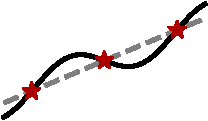
\includegraphics[width=\linewidth]{fig/fp.pdf}
\captionsetup{font={footnotesize}}
\caption{Fixed points of a map.}
\label{fig:fp}
\end{wrapfigure}

\begin{definition}
  A \emph{fixed point} $y^\star\in\R^n$ of a map
  $g:\R^n\rightarrow\R^n$ is where $g(y^\star) = y^\star$.
  \label{def:fixed}
\end{definition}

Continuous fixed-point problems as in \cref{def:fixed}
are ubiquitous in engineering and science and
amortizing their solutions is an activate research area.
Let $\gR(y)\defeq g(y)-y$ be the \emph{fixed-point residual}
with squared norm $\gN(y)\defeq \|\gR(y)\|_2^2$.
Fixed-point computations are connected to continuous
unconstrained optimization as any fixed-point problem can be
transformed into \cref{eq:opt} by optimizing the
residual norms with:
\begin{equation}
  y^\star(x)\in\argmin_y \gN(y),
  \label{eq:fixed-point-opt}
\end{equation}
and conversely \cref{eq:opt} can be transformed into
a fixed-point problem via first-order optimality
to find the fixed-point of
$\nabla f(y) - y = 0$.
Thus methods that to amortize the solutions to \cref{eq:opt}
can help amortize the solutions
to fixed-point computations \cref{def:fixed}.

\textbf{Solving and accelerating fixed-point computations.}
Fixed points can be found with \emph{fixed-point iterations}
$y^{t+1}\defeq f(y^t)$ or by using
\emph{Newton's root-finding method} on the
fixed-point residuals with
\begin{equation}
  y^{t+1}\defeq y^t - \left(\D_y g(y^t)\right)^{-1} g(y^t).
  \label{eq:newton}
\end{equation}
These methods can also be \emph{accelerated} by using
a sequence of past iterates instead of just the most
recent iterate.
\emph{Anderson acceleration} methods
\citep{anderson1965iterative,walker2011anderson,zhang2020globally}
are standard and generate updates that combine the
previous $M+1$ iterates $\{y^i\}_{i=t-M}^t$  with an update of the form
\begin{equation}
  \label{eq:aa-update}
  {\rm AA\_Update}^t(\{y_i\}, \alpha, \beta) \defeq
  \beta \sum_{i=0}^M \alpha_i g(y^{t-M+i}) +
  (1-\beta)\sum_{i=0}^M\sum_{i=0}^M \alpha_i y^{t-M+i},
\end{equation}
where $\beta\in[0,1]$ is a coefficient that controls
whether the iterates or application of $g$ on the iterates
should be used, and $\alpha\in\R^{M+1}$ where $1^\top\alpha=1$
are the coefficients used to combine the previous iterates.
A basic AA method sets $\beta=1$ and solves
\begin{equation}
  \label{eq:aa-alpha}
  \alpha^\star\defeq \argmin_\alpha \|\gR(y^i)\alpha\|_2\; \subjectto\; 1^\top \alpha = 1
\end{equation}
for $i\in\{t-M,t\}$ with least squares.
Other methods such as
\emph{Broyden's method} \citep{broyden1965class} can
also accelerate fixed-point computations by turning them
into root-finding problems.

\subsubsection{Neural fixed-point acceleration (NeuralFP) and conic optimization with the splitting cone solver (NeuralSCS)}
\label{sec:apps:neural-fp}
\emph{Neural fixed-point acceleration} \citep{venkataraman2021neural}
proposes a semi-amortized method for computing fixed-points
and use it for convex cone programming.
Representing a latent state at time $t$ with $\hat h^t$,
they parameterize the initial iterate
$\left(\hat y^0, \hat h^0\right) = {\rm init}_\theta(x)$
with an \emph{initialization model} ${\rm init_\theta}$
and perform the fixed-point computations
\begin{equation}
  \begin{aligned}
    \tilde x^{t+1} &= f(\hat y^t; x) \\
    \left(\hat y^{t+1},\hat h^{h+1}\right) &= {\rm acc}_\theta(\hat y^t, \tilde x^{t+1}, \hat h^t)
  \end{aligned}
  \label{eq:neural-fp}
\end{equation}
using an \emph{acceleration model} ${\rm acc_\theta}$
that is typically a recurrent model that predicts the
next iterate given the past sequence of iterates.
\citet[Prop. 1]{venkataraman2021neural} discuss how
this model captures standard AA as an instance
by setting the models equal to the standard update
that doesn't use learning.
They learn this model to amortize \cref{eq:fixed-point-opt}
over a distribution of contexts $p(x)$ with an objective-based loss
that solves
\begin{equation}
  \argmin_\theta \E_{x\sim p(x)} \sum_{t=0}^K \gN(\hat y^t_\theta(x)),
  \label{eq:neural-fp-loss}
\end{equation}
where the fixed-point residual norm $\gN$ is scaled by a
context-specific \emph{normalization factor}.

\emph{NeuralSCS} \citep{venkataraman2021neural} applies this
neural fixed-point acceleration to solve
\emph{constrained convex cone programs}
solved by the splitting cone solver (SCS)
\citep{o2016conic}
of the form
\begin{equation}
  \label{eq:cone_problem}
\begin{aligned}[c]
  & \minimize\; c^{T}x \\
  & \st \; Ax + s = b \\
  & \qquad (x,s) \in \mathbb{R}^n \times \mathcal{K}
\end{aligned}
\qquad
\begin{aligned}[c]
  & \maximize\; -b^{T}y \\
  & \st\; -A^{T}y + r = c \\
  & \qquad (r,y) \in \{0\}^n \times \mathcal{K}^*
\end{aligned}
\end{equation}
where $x \in \mathbb{R}^n$ is the primal variable, $s \in
\mathbb{R}^m$ is the primal slack variable, $y \in \mathbb{R}^m$ is
the dual variable, and $r \in \mathbb{R}^n$ is the dual residual. The
set $\mathcal{K} \in \mathbb{R}^m$ is a non-empty convex cone with
dual cone $\mathcal{K}^* \in \mathbb{R}^m$.
where $x \in \mathbb{R}^n$ is the primal variable, $s \in
\mathbb{R}^m$ is the primal slack variable, $y \in \mathbb{R}^m$ is
the dual variable, and $r \in \mathbb{R}^n$ is the dual residual. The
set $\mathcal{K} \in \mathbb{R}^m$ is a non-empty convex cone.
SCS uses the \emph{homogeneous self-dual embedding} to view
\cref{eq:cone_problem} as a fixed-point computation
over $\gZ=\R^{n\times m\times 1}$ with a scalar-valued scaling factor
as the last component.

NeuralSCS proposes a semi-amortized model to predict
the solution to the fixed point of the self-dual embedding
that solves \cref{eq:cone_problem}.
Their semi-amortized model $\hat z_\theta(\phi)$ takes
a context $\phi$ as the input and outputs a solution to the
self-dual embedding by composing the SCS iterations $f$ with
the learned fixed-point acceleration modules
(${\rm init}_\theta,{\rm acc}_\theta$).

\textbf{Summary.}
$\gA_{\rm NeuralSCS}\defeq\left(\gN, \gZ, \phi, p(\phi), \hat z_\theta, \gL_{\rm obj}^\Sigma\right)$

\subsubsection{Neural acceleration for matrix factorization (NeuralNMF)}
\citet{sjolund2022graphbased} use semi-amortized neural acceleration
to find low-rank factorizations of an input matrix $V$ of the form:
\begin{equation}
  V\approx WH^\top, \qquad W\geq 0, H\geq 0,
  \label{eq:nmf}
\end{equation}
where the basis matrix $W\in\R^{m\times r}$ and
mixture matrix $H\in\R^{n\times r}$ are elementwise
non-negative matrices of rank $r\leq\min(m,n)$.
Let $Z=(W,H)$. Taking the norm of the residual of \cref{eq:nmf}
leads to the optimization formulation
\begin{equation}
  Z^\star(V)\in \argmin_{W,H\geq 0} \gN_{\rm NMF}(W, H; V) \qquad
  \gN_{\rm NMF}(W, H; V)\defeq \frac{1}{2}\|WH^\top - V\|_F^2,
  \label{eq:nmf-opt}
\end{equation}
which can be solved with ADMM \citep{boyd2011distributed}.
Given a distribution over input matrices $V$,
\citet{sjolund2022graphbased}, augment a base ADMM
method with transformer-based initialization and
acceleration modules.
This semi-amortized model is learned with an
objective-based loss and unrolls through
the ADMM iterations for learning.

\textbf{Summary.}
$\gA_{\rm NeuralNMF}\defeq\left(\gN_{\rm NMF}, \gZ, V, p(V), \hat Z_\theta, \gL_{\rm obj}^\Sigma\right)$

\subsubsection{HyperAnderson acceleration and
  deep equilibrium models (HyperDEQ)}
\label{sec:apps:deq}

\citet{bai2022neural} similarly proposes a semi-amortized
method for computing fixed-points and use it to
improve \emph{Deep equilibrium (DEQ) models}
\citep{bai2019deep,bai2020multiscale,gurumurthy2021joint}.
Their learned variant of AA, called \emph{HyperAnderson acceleration}
uses models that predict the initial point $\hat y^0_\theta(x)$
and coefficients $\alpha_\theta(x; G)$ and $\beta_\theta(x; G)$
and result in iterations of the form
\begin{equation}
  G^{t+1}_\theta, \hat y^{t+1}_\theta \defeq
  {\rm AA\_Update}(\{\hat y^t_\theta\},
    \alpha^t_\theta(x; G^t_\theta), \beta^t_\theta(x, G^t_\theta)),
  \label{eq:hyperaa}
\end{equation}
where $G^t\defeq \gR(x^t)$ is the fixed-point residual at
iteration $t$ and the model's final prediction is
$\hat y_\theta(x)\defeq x^K$.
Learning is performed by optimizing a summed regression-based loss
that encourages the fixed-point iterations to converge
as fast as possible by optimizing
\begin{equation}
  \argmin_\theta \gL_{\rm HyperAA}(\hat y_\theta) \qquad \gL_{\rm HyperAA}(\hat y_\theta) \defeq \E_{x\sim p(x)} \sum_{t=0}^K w_t \|y^\star - \hat y_\theta^t\|_2^2 + \Omega(\alpha^t),
  \label{eq:hyperaa-loss}
\end{equation}
where $\Omega$ is a regularizer on $\alpha^t$ that is annealed
to equal zero by the end of training and the
weights $(w_t)$ are set to be monotonically increasing to
penalize the later iterations for not reaching the fixed point.

\emph{Deep equilibrium (DEQ) models} \citep{bai2019deep,bai2020multiscale}
investigate implicit layers that parameterize and solve
fixed-point computations and have been a flagship for
``infinite depth'' vision and language models.
Given an input $x\in\gX$, such as an image or language sequence
to process, a DEQ model finds a fixed point $y^\star(x)$
of $g_\varphi(y; x)$ to make a prediction for a task,
such as regression or classification.
This fixed-point problem can again be interpreted as
finding the minimum norm of the residual
$\gN(y; x)\defeq ||y-g_\varphi(y;x)||_2^2$
as
\begin{equation}
  y^\star(x)\in \argmin_x \gN(y; x).
  \label{eq:deq-opt}
\end{equation}
\citet{bai2022neural} propose to use the HyperAnderson Acceleration
model and loss to semi-amortize DEQs by learning the initial
iterate and AA update coefficients, resulting in a setup of the form
$\gA_{\rm HyperDEQ}\defeq(\gN, \gY, \gX, p(x), \hat y_\theta, \gL_{\rm HyperAA})$.

\subsubsection{Comparing NeuralFP and HyperAA}
Neural fixed-point acceleration (NeuralFP) by \citet{venkataraman2021neural}
and
HyperAnderson Acceleration (HyperAA) by \citet{bai2022neural}
can both generally be applied to semi-amortize
fixed-point computations by parameterizing updates
based on Anderson Acceleration, even though they are
instantiated and evaluated on very different classes of
fixed-point computations.
Here we briefly compare the methods:
\vspace{8mm}

\noindent
\begin{minipage}[t]{0.5\textwidth}
\noindent\textbf{Neural fixed-point acceleration}
\begin{itemize}[leftmargin=*,noitemsep]
\item Learn the initial iterate
\item Learn the entire update
\item Use an objective-based loss
\end{itemize}
\end{minipage}
\begin{minipage}[t]{0.5\textwidth}
\textbf{HyperAnderson Acceleration}
\begin{itemize}[leftmargin=*,noitemsep]
\item Learn the initial iterate
\item Learn $\alpha,\beta$ for the update
\item Use an regression-based loss
\end{itemize}
\end{minipage}

\subsubsection{RLQP by \citet{ichnowski2021accelerating}}
\label{sec:apps:qprl}
RLQP \citep{ichnowski2021accelerating} amortizes solutions to constrained
convex quadratic optimization problems of the form
\begin{equation}
  x^\star(\phi)\in \argmin_x \frac{1}{2} x^\top Px+ q^\top x\; \subjectto\; l\leq Ax\leq u,
  \label{eq:qp}
\end{equation}
where $x\in\R^n$ is the \emph{domain} of the optimization problem
and $\phi=\{P,q,l,A,u\}$ is the \emph{context} or \emph{parameterization}
(from a larger space $\phi\in\Phi$)
of the optimization problem with $P\succ 0$ (symmetric positive semi-definite).
They build on the OSQP solver \citep{stellato2018osqp} for these
optimization problems, which is based on operator splitting.
Without over-relaxation, the core of OSQP uses updates
that first solve the system
\begin{equation}
  \begin{bmatrix}
    P+\sigma I & A^\top \\
    A & -{\rm diag}(\rho^t)^{-1} \\
  \end{bmatrix}
  \begin{bmatrix}
    x^{t+1} \\
    v^{t+1}
  \end{bmatrix}
  =
  \begin{bmatrix}
    \sigma x^t - q \\
    z^t - {\rm diag}(\rho^t)^{-1} y^t
  \end{bmatrix}
  \label{eq:osqp-system}
\end{equation}
and then updates
\begin{equation}
  \begin{aligned}
  \tilde z^{t+1} &\defeq z^t+{\rm diag}(\rho^t)^{-1}(v^{t+1}-y^t) \\
  z^{t+1} &\defeq \Pi\left(\tilde z^{t+1}+{\rm diag}(\rho^t)^{-1}y^t\right) \\
  y^{t+1} &\defeq x^t + {\rm diag}(\rho)\left(\tilde z^{t+1}-z{t+1}\right),
  \end{aligned}
  \label{eq:osqp-update}
\end{equation}
where $y,v$ are dual variables,
$z,\tilde z$ are auxiliary operator splitting variables,
$\sigma$ is a regularization parameter, and
$\rho^t\in\R^m_+$ is a step-size parameter.
We combine all of the variables into a state
$s\defeq(y, \lambda, \tilde z, z)$ living in
$s\in\gS$ and write the update as
$s^{t+1}\defeq{\rm OSQP\_UPDATE}(s^t, \rho^t)$.

RLQP proposes to use these OSQP iterates as a
semi-amortized model with the iterates
$\{s^t, \rho^t\}$. The propose to only parameterize and
learn to predict the step size
$\rho^{t+1}\defeq \pi_\theta(s^t)$, with a
neural network amortization model $\pi_\theta$.
They model the process of predicting the optimal $\rho$ as
an MDP and define a reward $R_{\rm RLQP}(s, \rho)$ that
is $-1$ if the QP is not solved
(based on thresholds of the primal and dual residuals)
and $0$ otherwise, \ie each episode rolls
out the OSQP iterations with a policy predicting
the optimal step size.
They solve this MDP with TD3 by \citet{fujimoto2018td3}
to find the parameters $\theta$.

\textbf{Summary.}
$\gA_{\rm RLQP}\defeq (R_{\rm RLQP}, \gS\times\R^m_+, \Phi, p(\phi), \pi_\theta, \gL^{\rm RL}_{\rm obj})$


\subsection{Amortized policy learning for control
  and reinforcement learning}
\label{sec:apps:ctrl}

\begin{figure}[t]
  \centering
  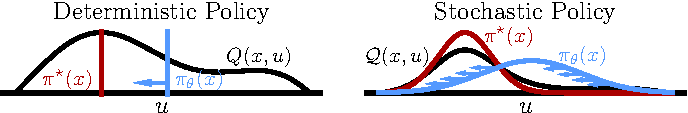
\includegraphics[width=\textwidth]{fig/ctrl.pdf}
  \caption{
    Many policy learning methods amortize
    optimization problem over the $Q$-values.
    Given a fixed input state $x$,
    the policy $\pi_\theta(x)$ predicts the
    maximum value $\pi^\star(x)$.
    A stochastic policy predicts
    a distribution that minimizes some probabilistic distance to
    the $Q$-distribution, such as the expected
    value or KL.
  }
  \label{fig:ctrl}
\end{figure}

Many control and reinforcement learning methods amortize the
solutions to a control optimization problem as illustrated in
\cref{fig:overview,fig:ctrl}.

\textbf{Distinction.} This section is on \emph{amortization for
reinforcement learning and control} and \emph{not} the
different direction of using \emph{reinforcement learning
for amortization} that we discuss in
\cref{sec:learning:rl} for parameter learning.

\subsubsection{Background}
\textbf{Preliminaries in Markov decision processes.}
\begin{definition}
  We represent a \emph{Markov decision process} (MDP) with
  $\gM\defeq(\gX, \gU, p, r)$,
  where $\gX$ are the continuous \emph{states},
  $\gU$ are the continuous \emph{actions} or \emph{controls},
  $p(x' \mid x, u)$ is the \emph{transition dynamics}
  (also referred to as the \emph{system}, \emph{model},
  or \emph{world model}),
  which is a \emph{Markov kernel} providing
  the probability the next state $x'$
  given the current state-action $(x, u)$,
  and $r: \gX\times\gU$ is the \emph{reward function}.
\end{definition}
We scope to methods that control a
fully-observable and continuous MDP.
A \emph{policy} $\pi$ that \emph{controls}
the MDP provides a distribution over actions to sample from
for every state $x$ and induces \emph{state} and
\emph{state-control marginals} $\rho_t^\pi(\cdot)$ for each
time step $t$, which can be constrained to start from an initial
state $x_0$ as $\rho_t(\cdot|x)$.
In the non-discounted, infinite-horizon case
an \emph{optimal policy} $\pi^\star$ maximizes the reward over
rollouts of the MDP with
\begin{equation}
  \pi^\star(x)\in \argmax_\pi \E_{x\sim p_{\rm init}(x)} V^\pi(x)
  \qquad
  V^\pi(x)\defeq \sum_t \E_{(x_t, u_t)\sim\rho_t^\pi(\cdot\mid x)} r(x_t, u_t),
  \label{eq:pistar}
\end{equation}
where $p_{\rm init}$ is the \emph{initial state distribution}
and $V^\pi(x)$ is the expected \emph{value} of a policy $\pi$
starting from a state $x$ and that is taken over all possible
future rewards induced by the stochastic policy and dynamics.
Given the \emph{action-conditional value} $Q$ of a policy
defined by
\begin{equation}
  Q^\pi(x, u)\defeq r(x, u) + \E_{x'\sim p(\cdot|x,u)}\left[V^\pi(x')\right].
  \label{eq:Q}
\end{equation}
In the deterministic setting with a fixed $Q$ function,
an optimal policy can be obtained by solving the
\emph{max-Q} optimization problem
\begin{equation}
  \pi^\star(x) \in \argmax_u Q(x, u),
  \label{eq:Q-opt}
\end{equation}
which is the form we will often use to interpret many
control and reinforcement learning methods
as amortized optimization.
Instead of amortizing the solution to \cref{eq:Q-opt},
methods such as \citet{lowrey2018plan,ryu2019caql}
explicitly solve the max-Q problem.

\textbf{Control of deterministic MDPs with deterministic policies.}
If all of the components of the MDP are known,
no learning needs to be done to obtain an optimal policy
and standard \emph{model predictive control} (MPC) methods often work well.
In \emph{deterministic MDPs}, the dynamics are deterministic,
which we write as $x'\defeq p(x, u)$.
These can be solved with deterministic policies,
which turns the expected value and marginal distributions
into Dirac delta distributions that can be computed with single rollout.
An optimal controller from an initial state $x_1$ can thus
be obtained by solving the \emph{finite-horizon} problem over the
(negated) value approximated with a horizon length of
$H$ timesteps with
\begin{equation}
  u^\star_{1:H}(x_1) \defeq \argmin_{u_{1:H}} \sum_t C_t(x_t, u_t)\; \subjectto\; x_{t+1}=p(x_t, u_t),
  \label{eq:mpc}
\end{equation}
where the \emph{cost} $C$ at each time is usually the negated reward
$C_t(x_t, u_t)\defeq -r(x_t, u_t)$.
\Cref{eq:mpc} induces the policy $\pi(x)\defeq u^\star_1(x)$ that
solves the MDP if the horizon $H$ is long enough.
Using a \emph{terminal cost} at the end of the horizon can
also give the controller information about how the system will
perform beyond the finite-horizon rollouts being used,
for example with
$C_H(x_H, u_H)\defeq -Q^\pi(x_H, u_H)$.

\textbf{Reinforcement learning when the dynamics aren't known.}
Optimal control methods work well when the dynamics $p$
of the MDP are known, which is an unfortunately strong
assumption in many settings where we are only able to
sample from the system.
In these settings \emph{reinforcement learning} (RL)
methods thrive and solve the MDP given access to
\emph{only} samples from the dynamics.
While summarizing all of the active RL methods is out-of-scope
for this tutorial, the core of these methods is typically on
1) \emph{policy evaluation} to estimate the \emph{value}
of a policy given only samples from the system, and
2) \emph{policy improvement} to improve the policy
using the value estimation.

\textbf{Extensions in stochastic control.}
The max-Q problem in \cref{eq:Q-opt} can be extended to the
stochastic optimization settings we briefly covered in
\cref{sec:extensions:sto} when the policy $\pi$
represents a \emph{distribution} over the action space $\gU$.
The most common objectives for stochastic policies are
1) the expected $Q$-value under the policy with
\begin{equation}
  \pi^\star(x) \in \argmax_{\pi\in\Pi} \gE_Q(\pi; x) \qquad \gE_\gQ(\pi; x)\defeq \E_{u\sim\pi(\cdot)} Q(x,u),
  \label{eq:Q-opt-sto-exp}
\end{equation}
or 2) the KL distance
\begin{equation}
  \pi^\star(x) \in \argmin_{\pi\in\Pi} \D_\gQ(\pi; x) \qquad \D_\gQ(\pi; x)\defeq \kl{\pi(\cdot)}{\gQ(x, \cdot)},
  \label{eq:Q-opt-sto-kl}
\end{equation}
where $\gQ(x, \cdot)\propto \exp\left\{Q(x, \cdot)/\alpha\right\}$
is a $Q$-distribution induced by the $Q$ values that is
inversely scaled by $\alpha\in\R_+$.
The policy $\pi$ is usually represented as the parameters of a distribution
and thus $\Pi$ becomes the space of these parameters.
In most cases we take $\pi$ to be a Gaussian $\gN(\mu, \Sigma)$
with a diagonal covariance $\Sigma$ and thus we thus we can
turn \cref{eq:Q-opt-sto-exp,eq:Q-opt-sto-kl} into unconstrained continuous
optimization problems of the form \cref{eq:opt} by
projecting onto the Gaussian parameters.
We will see that stochastic value gradient methods such as \citet{heess2015learning}
often amortize \cref{eq:Q-opt-sto-exp}, while
\citet{levine2013guided,haarnoja2018soft} propose methods
that build on \cref{eq:Q-opt-sto-kl}, often adding additional
softening and entropic terms to encourage the policy
and value estimate to explore more and not converge too
rapidly to a suboptimal minima.
Lastly, we note again that the smoothing that the policy performs in
\cref{eq:Q-opt-sto-exp} is nearly identical to the objective
smoothing considered in \cref{sec:smooth}, except in that setting
the variance of the smoother remains fixed.

\textbf{Connecting stochastic control back to deterministic control.}
We show that taking stochastic policies to be Dirac delta distributions
in \cref{eq:Q-opt-sto-exp,eq:Q-opt-sto-kl} recovers the solutions to the
deterministic control problem in \cref{eq:Q-opt}.
Taking a larger classes of policy distributions, such as
Gaussians, can then be interpreted as smoothing the $Q$
values to avoid 1) falling into poor local optima and
2) instable regions where only a few actions have
high value, but the rest have poor values.
For the following, let $\delta_u(\cdot)$ be Dirac delta
distribution with a parameter $u\in\R^n$ indicating the
location of the mass.

\begin{proposition}
  Let $\pi$ be a Dirac delta distribution $\delta_u(\cdot)$.
  Then the solution $\pi^\star(x)$ to the expected $Q$ problem in
  \cref{eq:Q-opt-sto-exp} is the solution to the deterministic
  max-$Q$ problem in \cref{eq:Q-opt}.
\end{proposition}

\begin{proof}
  Let $\Pi=\R^n$ be the parameter space of $\pi$ and transform
  \cref{eq:Q-opt-sto-exp} to optimize over it:
  \begin{equation}
  \pi^\star(x) \in \argmax_{u\in\R^n} \E_{\tilde u\sim\delta_u(\cdot\mid x)}{Q(x, \tilde u)}.
  \label{eq:exp-dirac-opt}
  \end{equation}
  The expectation over the Dirac evaluates to
  \begin{equation}
    \E_{\tilde u\sim\delta_u(\cdot\mid x)}{Q(x, \tilde u)} = Q(x,u)
    \label{eq:exp-expansion}
  \end{equation}
  and thus \cref{eq:exp-dirac-opt}
  which is the max-$Q$ operation in \cref{eq:Q-opt}.
\end{proof}

\noindent Similarly for the for the KL problem in \cref{eq:Q-opt-sto-kl}:
\begin{proposition}
  Let $\pi$ be a Dirac delta distribution $\delta_u(\cdot)$.
  Then the solution $\pi^\star(x)$ to the KL problem in
  \cref{eq:Q-opt-sto-kl} is the solution to the deterministic
  max-$Q$ problem in \cref{eq:Q-opt}.
\end{proposition}

\begin{proof}
  Let $\Pi=\R^n$ be the parameter space of $\pi$ and transform
  \cref{eq:Q-opt-sto-kl} to optimize over it:
  \begin{equation}
  \pi^\star(x) \in \argmin_{u\in\R^n} \kl{\delta_u(\cdot)}{\gQ(x, \cdot)}.
  \label{kl-dirac-opt}
  \end{equation}
  Expanding the KL distance then gives the density of $\gQ$ at the mass:
  \begin{equation}
    \begin{aligned}
      \kl{\delta_u(\cdot)}{\gQ(x, \cdot)}
      & = \E_{\tilde u\sim \delta_u(\cdot)} \left[ \log{\delta_u(\tilde u)} - \log \gQ(x,\tilde u)\right] \\
      & = -\log \gQ(x,u)+C \\
      & = -\log \frac{1}{\gZ_x}\exp\left\{Q(x,u)\right\} + C\\
      & = -Q(x, u) + \log \gZ_x + C \\
    \end{aligned}
    \label{eq:kl-expansion}
  \end{equation}
  where $C$ is a constant that does not depend on $u$,
  $\gQ(x,u)$ is the density at $u$, and
  $\gZ_x$ is the normalization constant for $\gQ(x,\cdot)$
  that does not depend on $u$.
  Putting \cref{eq:kl-expansion} back into
  \cref{kl-dirac-opt} and removing the constants that
  do not depend on $u$ gives
  \begin{equation}
  \pi^\star(x)\in \argmin_{u\in\R^n} -Q(x,u),
  \end{equation}
  which is the max-$Q$ operation in \cref{eq:Q-opt}.
\end{proof}

\subsubsection{Behavioral cloning and imitation learning}
We will start in the setting where regression-based amortization
is done to predict the solution of a controller that
solves \cref{eq:pistar}.
In these settings, we have access to a controller, or samples from it,
that uses traditional methods, and \emph{not} learning,
to solve \cref{eq:pistar}, and we either know
the true dynamics or form an approximation to them
that the control is done on top of.
We typically have access to these solutions as samples
from a policy $\pi^\star(x)$ that provides the solution
to the max-Q problem in \cref{eq:Q-opt} that we want to
do regression-based amortization onto.
In some settings these methods also use the
optimal finite-horizon sequence $u^\star_{1:H}(x)$
from a solution to \cref{eq:mpc}.

Imitation learning methods such as behavioral cloning can be
seen as a regression-based amortization
that seek to distill, or clone,
the expert's behavior into a learned model $\pi_\theta(x)$
that predicts the expert's action given the state $x$.
Deterministic BC methods often regress onto the expert's
state-action pairs $(x, \pi^\star(x))$
sampled some distribution of states $p(x)$ with
\begin{equation}
  \argmin_\theta \E_{x\sim p(x)} \|\pi^\star(x)-\pi_\theta(x)\|_2^2,
  \label{eq:bc}
\end{equation}
where, for example, the model $\pi_\theta$ could
be a neural network.
Thus BC in this setting performs regression-based amortization
$\gA_{\rm BC}\defeq (-Q, \gU, \gX, p(x), \pi_\theta, \gL_{\rm reg})$.
Extensions from this setting could include when
1) the model $\pi_\theta$ is a sequence model that
predicts the entire sequence $u^\star_{1:H}$, and
2) the MDP or policy is stochastic and
\cref{eq:bc} turns into an amortized maximum likelihood
problem rather than a regression problem.

\textbf{Warning.}
One crucial difference between behavioral cloning
and all of the other applications that we consider
is that in behavioral cloning, we also may not know
the original objective that the expert solves.
We assume that an optimal objective
exists for the purposes of seeing it as regression-based
amortization.
Settings such as inverse control and RL
explicitly recover the expert's objective, but are
beyond the scope of our amortization focus.

\subsubsection{The deterministic policy gradient}
The policy learning of many model-free actor-critic
reinforcement learning algorithms on continuous spaces
can be seen as objective-based amortization of the
max-$Q$ operation in \cref{eq:Q-opt}.
This includes the policy improvement step for
deterministic policies as pioneered by the
deterministic policy gradient (DPG) by \citet{silver2014dpg},
deep deterministic policy gradient (DDPG) by \citet{lillicrap2015continuous},
and and twin delayed DDPG (TD3) by \citet{fujimoto2018td3}.
All of these methods interweave
1) \emph{policy evaluation} to estimate the
state-action value $Q^{\pi_\theta}$ of the current policy
$\pi_\theta$, and
2) \emph{policy improvement} to find the policy
that best-optimizes the max-Q operation with
\begin{equation}
  \argmax_\theta \E_{x\sim p(x)} Q(x, \pi_\theta(x)).
  \label{eq:dpg-loss}
\end{equation}

\textbf{Summary.}
The DPG family of methods perform objective-based
amortization of the max-$Q$ optimization problem with
$\gA_{\rm DPG}\defeq (-Q, \gU, \gX, p(x), \pi_\theta, \gL_{\rm obj})$.

\subsubsection{The stochastic value gradient and soft actor-critic}
This amortization viewpoint can be extended to \emph{stochastic} systems
and policies that use the \emph{stochastic value gradient} (SVG)
and covers a range of model-free to model-based method depending on
how the value is estimated
\citep{byravan2019imagined,hafner2019dream,byravan2021evaluating,amos2021model}.
As observed in
\citet{haarnoja2018soft,amos2021model},
the policy update step in the soft actor-critic
can also be seen as a model-free
stochastic value gradient with the value estimate
regularized or ``softened'' with an entropy term.
These methods learn policies $\pi_\theta$ that
amortize the solution to a stochastic optimization
problem, such as \cref{eq:Q-opt-sto-exp,eq:Q-opt-sto-kl},
over some distribution of states $p(x)$, such as the
stationary state distribution or an approximation of it
with a replay buffer.
Taking the expected value under the policy gives
the policy loss
\begin{equation}
  \argmax_\theta \gL_{\rm SVG,\gE}(\pi_\theta) \qquad \gL_{\rm SVG,\gE}(\pi_\theta)\defeq \E_{x\sim p(x)} \E_{u\sim\pi(\cdot|x)} Q(x, u),
  \label{eq:svg-loss-exp}
\end{equation}
and taking the minimum KL distance gives the policy loss
\begin{equation}
  \argmin_\theta \gL_{\rm SVG,KL}(\pi_\theta) \qquad \gL_{\rm SVG,KL}(\pi_\theta)\defeq \E_{x\sim p(x)} \kl{\pi_\theta(\cdot\mid x)}{\gQ(x, \cdot)},
  \label{eq:svg-loss-kl}
\end{equation}
which softens the policy and value estimates with an entropy regularization
as in \citet{haarnoja2018soft,amos2021model}.
\Cref{eq:svg-loss-kl} can be seen as an entropy-regularized value
estimate by expanding the KL
\begin{equation}
  \E_{x\sim p(x)} \kl{\pi_\theta(\cdot\mid x)}{\gQ(x, \cdot)} =
  \E_{x\sim p(x)} \E_{u\sim \pi(u\mid x)} \left[ \alpha\log(\pi(u\mid x)) - Q(x, u) \right].
\end{equation}

\textbf{Summary.}
The policy update of methods based on the SVG and SAC perform
objective-based amortization of a stochastic control
optimization problem with
\begin{equation*}
\gA_{\rm SVG}\defeq (\D_\gQ\;\mathrm{or}\;-\gE_Q, \gP(\gU), \gX, p(x), \pi_\theta, \gL_{\rm KL}).
\end{equation*}

\textbf{SVG-based amortization for model-free and model-based methods.}
SVG-based policy optimization provides a spectrum of model-free
to model-based algorithms depending on if the value estimate is
approximated in a model-free or model-based way, \eg with rollouts
of the true or approximate dynamics.
\citet{heess2015learning} explored this spectrum and proposed
a few key instantiations.
\citet{byravan2019imagined,amos2021model} use learned
models for the value approximation.
The variation in \citet{hafner2019dream} amortizes a model-based
approximation using the \emph{sum} of the value estimates
of a model rollout.
\citet{henaff2019model} explore uncertainty-based regularization to
amortized policies learned with value gradients.
\citet{xie2020latent} consider hierarchical amortized optimization
that combine a higher-level planner based on CEM with a
lower-level fully-amortized policy learned
with stochastic value gradients.
\citet{byravan2021evaluating} perform a large-scale evaluation of
amortization methods for control and study algorithmic variations
and generalization capabilities, and consider methods based on
the stochastic value gradient and behavioral cloning.

\subsubsection{PILCO by \citet{deisenroth2011pilco}}
PILCO is an early example that uses gradient-based
amortization for control.
They assume that only samples from the dynamics model are
available, fit a Gaussian process to them, and then use that
to estimate the finite-horizon $Q$-value of a
deterministic RBF policy $\pi_\theta$.
The parameters $\theta$ are optimized by taking gradient
steps to find the policy resulting in the maximum value
over some distribution of states $p(x)$, \ie
\begin{equation}
  \argmax_\theta \E_{x\sim p(x)} Q(x, \pi_\theta).
\end{equation}

\textbf{Summary.}
$\gA_{\rm PILCO}\defeq (-Q, \gU, \gX, p(x), \pi_\theta, \gL_{\rm obj})$

\subsubsection{Guided policy search (GPS)}
The GPS family of methods
\citep{levine2013guided,levine2014learning,levine2016end,montgomery2016guided}
fits an approximate dynamics model to data and then
amortizes the solutions of a controller that solves
the MPC problem in \cref{eq:mpc} within a local region of
the data to improve the amortization model.
Given samples of $\pi^\star$ from a controller that solves
\cref{eq:Q-opt-sto-kl},
GPS methods typically optimize the KL divergence between
the controller and these samples with
\begin{equation}
  \argmin_\theta \E_{x\sim p(x)} \kl{\pi_\theta(\cdot\mid x)}{\pi^\star(\cdot\mid x)}
  \label{eq:gps}
\end{equation}

\textbf{Summary.}
$\gA_{\rm GPS}\defeq (\D_\gQ, \gP(\gU), \gX, p(x), \pi_\theta, \gL_{\rm KL})$

\subsubsection{POPLIN by \citet{wang2019exploring}}
POPLIN explores behavioral cloning methods based on regression
and generative modeling and observes that the
parameter space of the amortized model is a reasonable
space to solve new control optimization problems over.
The methods discussed here

\textbf{Distillation and amortization.}
POPLIN first trains a fully-amortized
model on a dataset of trajectories with behavioral cloning
or generative modeling.
Here we only consider the BC variant trained with
$\gA_{\rm BC}$, which provides an \emph{optimal}
fully-amortized model $\pi_{\theta^\star}$.

\textbf{Control.}
Next they explore ways of using the learned policy
$\pi_{\theta^\star}$ to solve the model predictive
control optimization problem in \cref{eq:mpc}.
The \emph{POPLIN-A} variant (``A'' stands for ``action'')
uses $\pi_{\theta^\star}$ to predict an initial
control sequence $\hat u^0_{1:H}$ that is then passed as
an input to a controller based on the cross-entropy method
over the action space that uses a learned model on the trajectories.
The \emph{POPLIN-P} variant (``P'' stands for ``parameter'')
suggests that the \emph{parameter space} of the fully-amortized
model has learned useful information about the structure
of the optimal action sequences.
As an alternative to solving the MPC problem in \cref{eq:mpc}
over the action space,
POPLIN-P proposes to use CEM to find a
perturbation $\omega$ to the optimal parameters $\theta^\star$
that maximizes the value from a state $x$ with
\begin{equation}
  \omega^\star(x) \in \argmax_\omega Q(x, u;
    \pi_{\theta^\star+\omega}).
  \label{eq:POPLIN-P}
\end{equation}
Thus the action produced by
$\pi_{\theta^\star+\omega^\star}(x)$
is a solution the control problem in \cref{eq:mpc}
obtained by adapting the policy's parameters to the
state $x$.

\textbf{Summary.} POPLIN is an extension of
of behavioral cloning that amortizes control optimization
problems with
$\gA_{\rm POPLIN}\defeq (-Q, \gU, \gX, p(x), \pi_\theta, \gL_{\rm reg})$.
The initial phase is fully-amortized behavioral cloning.
The second fine-tuning phase can seen as semi-amortization
that learns only the initialization $\theta$ and
finds $\omega$ with CEM, with a regression-based loss $\gL_{\rm reg}$
that \emph{only} has knowledge of the initial model and does not include
the adaptation.

\subsubsection{The differentiable cross-entropy method by \citet{amos2019dcem}}

\begin{figure*}[t]
  \centering
  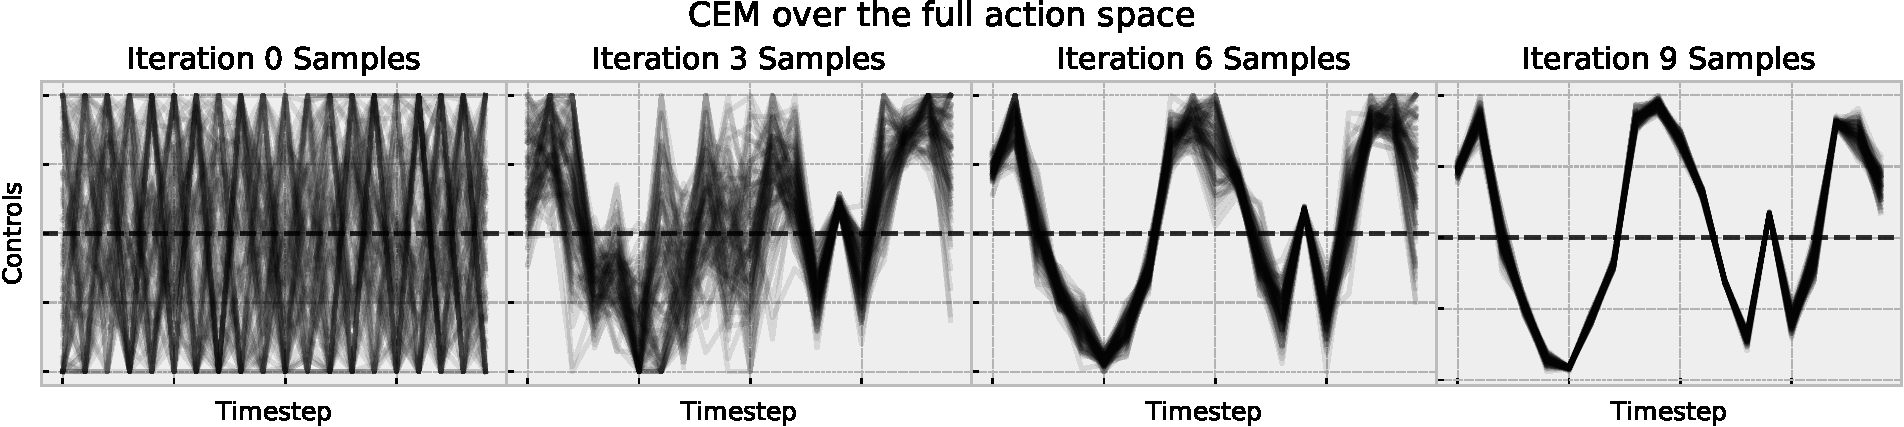
\includegraphics[width=\textwidth]{fig/dcem/cem-vis-full-space.pdf} \\[4mm]
  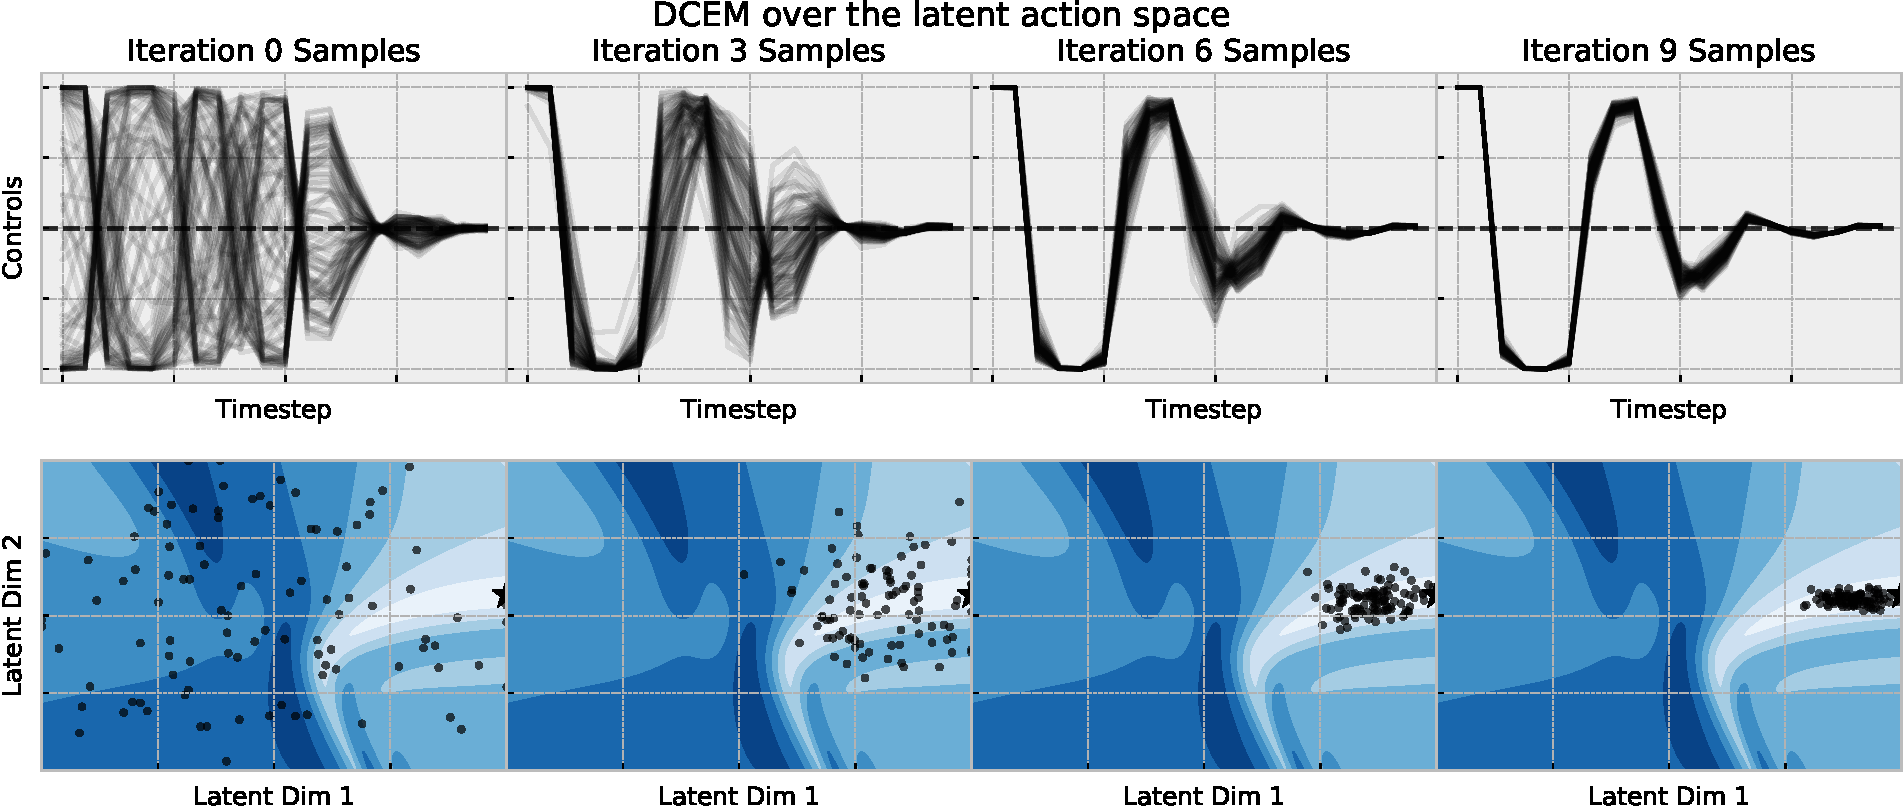
\includegraphics[width=\textwidth]{fig/dcem/cem-vis-latent-space.pdf}
  \caption{
    The differentiable cross-entropy method (DCEM) can be used
    to create semi-amortized controllers that learn a
    latent space $\gZ$ over control sequences.
    This visualization shows the samples that CEM and DCEM generate
    to solve the cartpole task starting from the same initial
    system state.
    The plots starting at the top-left show that CEM initially starts with
    no temporal knowledge over the control space whereas
    the latent space learned through DCEM generates a more
    feasible distribution over control sequences
    in each iteration that make them smooth and cyclic.
    The contours on the bottom show the controller's cost
    surface $C(z; x)$ for an initial state $x$ where
    the lighter colors show regions with lower costs.
  }
  \label{fig:dcem}
\end{figure*}

Differentiable control \citep{amos2018dmpc} is a budding area
of work with the goal of integrating controllers into
end-to-end modeling pipelines to overcome problems
such as objective mismatch \citep{lambert2020objective}.
The differentiable cross-entropy method (DCEM) was created
towards the goal of doing this with controllers
based on the cross-entropy method.
Otherwise, as in \citet{wang2019exploring}, CEM needs to be done as
a secondary step \emph{after} learning and the learning process is
not aware of the final policy that running CEM will induce.
The key step to differentiate through CEM is to make the
top-$k$ operation smooth and differentiable by using the
differentiable top-$k$ operation proposed in
\citet{amos2019limited} called the limited multi-label projection layer.

\citet{amos2019dcem} considers a semi-amortized learning setting
that learns a latent domain for control, which can be seen as
a similarly-motivated alternative to the parameter-space
control done in POPLIN.
The key piece of \emph{latent control}
is to learn a \emph{decoder} $\varphi_\theta:\gZ\rightarrow \gU^H$
that maps from a low-dimensional latent space $\gZ$ to the
$H$-step control space that solves \cref{eq:mpc}.
Learning a latent space is useful if there are many redundancies
and possibly bad local minimum on the original control space
$\gU^H$ that the latent space can get rid of.
Given an initial state $x_1$, the optimal latent representation
can be obtained by solving the control optimization problem
over $\gZ$ with
\begin{equation}
  \hat z_\theta(x_1)\in \argmin_{z\in\gZ} C_\theta(z; x_1)\;
  \label{eq:dcem-latent}
\end{equation}
where $C_\theta(z; x_1)$ is the expected cost of rolling out the
control sequence $u_{1:H}=\varphi(z)$ from the initial state
$x_1$, for example on deterministic systems $C$
could be the sum of negated rewards
\begin{equation}
  C(z; x) \defeq -\sum_{t=1}^H r(x_t, x_t)\;
  \subjectto\;x_{t+1}=p(x_t, u_t)\; {\rm and}\; x_{1:H}=\varphi_\theta(z)
  \label{eq:latent-cost}
\end{equation}
Solving \cref{eq:dcem-latent} with DCEM enables the optimal
solution $\hat z_\theta(x)$ to be differentiated with respect
to the parameters $\theta$ of the decoder $\varphi_\theta$.
The final predicted control sequence can be
obtained with the decoder
$\hat u_{1:H}(x; \theta)\defeq \varphi_\theta(\hat z_\theta(x))$
and the decoder can be learned by regressing
onto ground-truth control sequences $u^\star(x)$ with
\begin{equation}
  \argmin_\theta \gL_{\rm DCEM}(\hat u_{1:H}(\cdot; \theta)) \qquad \gL_{\rm DCEM}(\hat u_{1:H}(\cdot; \theta))\defeq \E_{x \sim p(x)}
  \|u^\star_{1:H}(x) - \hat u_{1:H}(x; \theta)\|_2^2.
\label{eq:dcem-loss}
\end{equation}
\Cref{fig:dcem} visualizes an example on the cartpole task
where this is able to learn a latent space that captures the
cyclic and smoothness structure of the optimal control
sequence space.

\textbf{Overview.} Learning a latent domain with the differentiable
cross-entropy method is a semi-amortization method with
$\gA_{\rm DCEM}\defeq (-Q, \gU, \gX, p(x), \pi_\theta, \gL_{\rm reg})$,
where the decoder $\varphi_\theta$ shows up from
the policy $\pi_\theta$ solving the latent
optimization problem with DCEM.

\subsubsection{Iterative amortized policy optimization (IAPO) by \citet{marino2020iterative}}
IAPO takes a probabilistic view and
starts with the observation that DPG and SVG methods
are amortized optimization problems with fully-amortized
models with an objective-based loss.
They then suggest to replace the model with an iterative
semi-amortized model where the policy $\pi_\theta$ internally
takes gradient steps on the actions of the underlying
control optimization problem, and explore this
semi-amortized policy in model-free and model-based
reinforcement learning settings.
Thus in the deterministic setting IAPO performs semi-amortized
optimization
$\gA_{\rm IAPO}\defeq (-Q, \gU, \gX, p(x), \pi_\theta, \gL_{\rm obj})$.

\section{Manifold extension: Amortized optimization on the sphere}
\label{sec:apps:sphere}

\begin{figure}
  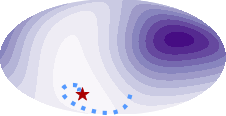
\includegraphics[width=0.25\textwidth]{fig/sphere/0.png}
  \hspace{-2.7mm}
  
\includegraphics[width=0.25\textwidth]{fig/sphere/1.png}
  \hspace{-2.7mm}
  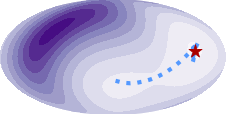
\includegraphics[width=0.25\textwidth]{fig/sphere/2.png}
  \hspace{-2.7mm}
  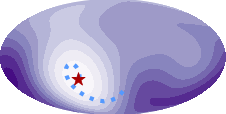
\includegraphics[width=0.25\textwidth]{fig/sphere/3.png} \\[-.8mm]
  
\includegraphics[width=0.25\textwidth]{fig/sphere/4.png}
  \hspace{-2.7mm}
  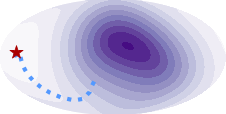
\includegraphics[width=0.25\textwidth]{fig/sphere/5.png}
  \hspace{-2.7mm}
  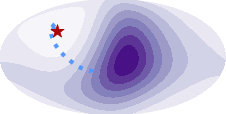
\includegraphics[width=0.25\textwidth]{fig/sphere/6.png}
  \hspace{-2.7mm}
  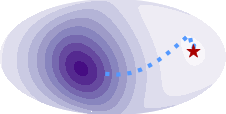
\includegraphics[width=0.25\textwidth]{fig/sphere/7.png} \\[-6mm]
  \begin{center}
    \cblock{73}{19}{134} $f(y; x)$ contours \;
    \cblock{170}{0}{0} Optimal $y^\star(x)$ \;
    \cblock{84}{153}{255} Predictions $\hat y_\theta(x)$ over training
  \end{center}
  \vspace{-3mm}
  \caption{We learn an amortized optimization model to
    predict the solution to optimization problems over the
    sphere. Here we show the predictions throughout training.}
  \label{fig:sphere}
\end{figure}


We conclude with a simple new demonstration that applies
the insights from amortized optimization to learn to solve
optimization problems over spheres of the form
\begin{equation}
  y^\star(x) \in \argmin_{y\in\gS^2} f(y; x),
  \label{eq:sphere-opt-con}
\end{equation}
where $\gS^2$ is the surface of the \emph{unit 2-sphere}
embedded in $\R^3$ as $\gS^2\defeq \{y\in\R^3 \mid \|y\|_2=1\}$
and $x$ is some parameterization of the function
$f: \gS^2\times\gX\rightarrow \R$.
\Cref{eq:sphere-opt-con} is relevant to physical and
geographical settings seeking the extreme values of a
function defined on the Earth or other spaces that can
be approximated with a sphere.

\textbf{Amortization objective.}
We first need to turn the constrained problem in \cref{eq:sphere-opt-con}
into an unconstrained optimization problem of the form
\cref{eq:opt}. In this setting, one way of doing this
is by using a projection:
\begin{equation}
  y^\star(x) \in \argmin_{y\in\R^3} f(\pi_{\gS^2}(y); x),
  \label{eq:sphere-opt-proj}
\end{equation}
where $\pi_{\gS^2}: \R^3\rightarrow \gS^2$ is the
Euclidean projection onto $\gS^2$, \ie,
\begin{equation}
  \begin{aligned}
    \pi_{\gS^2}(x)\defeq& \argmin_{y\in\gS^2} \|y-x\|_2 \\
     =& \;x/\|x\|_2.
  \end{aligned}
  \label{eq:pi}
\end{equation}

\textbf{$c$-convex functions on the sphere.}
We instantiate a synthetic class of
optimization problems defined on the sphere
using the $c$-convex functions from
\citet{cohen2021riemannian}:
\begin{equation}
  f(y; x) = {\textstyle \min_{\gamma}} \left\{\frac{1}{2} d(x,z_i)+\alpha_i\right\}_{i=1}^m
  \label{eq:rcpm}
\end{equation}
where $m$ components define the context
$x=\{z_i\} \cup \{\alpha_i\}$
with $z_i\in\gS^2$ and $\alpha_i\in\R$,
$d(x,y)\defeq \arccos(x^\top y)$ is the
Riemannian distance on the sphere in the
ambient Euclidean space, and
$\min_\gamma(a_1,\ldots,a_m)\defeq -\gamma\log\sum_{i=1}^m\exp(-a_i/\gamma)$
is a soft minimization operator
as proposed in \citet{cuturi2017soft}.
We sample $p(x)$ with $z_i\sim \gU(\gS^2)$,
uniformly from the sphere, and
$\alpha_i\sim\gN(0,\beta)$
with variance $\beta\in\R_+$.

\textbf{Amortization model.}
We next instantiate the model
$\hat y_\theta: \gX\rightarrow\R$
as a fully-connected MLP.
The predictions to \cref{eq:sphere-opt-con}
on the sphere can again be obtained by composing
the output with the projection
$\pi_{\gS^2}\circ \hat y_\theta$.

\textbf{Optimizing the gradient-based loss.}
Finally we choose to optimize the gradient-based loss $\gL_{\rm obj}$
as the objective and model are tractable and
easily differentiable.
\Cref{fig:sphere} shows the model's predictions
starting with the untrained model and finishing
with the trained model, showing that this setup
indeed enables us to predict the solutions to
\cref{eq:sphere-opt-con} with a single neural network
$\hat y_\theta(x)$ trained with the gradient-based loss.

\textbf{Summary.}
$\gA_{\rm sphere}\defeq (f\circ \pi_{\gS^2}, \R^3, \gX, p(x), \hat y_\theta, \gL_{\rm obj})$

\section{Discussion}
\label{sec:discussion}
Many of the specialized methods discuss tradeoffs and
limitations within the context of their application,
and more generally papers such as
\citet{chen2021learning,metz2021gradients}
provide even deeper probes into general paradigms for
learning to optimize.
Here we emphasize a few additional discussion points
around amortized optimization.

\subsection{Going beyond the known convergence rates of
  classical methods}
\label{sec:convergence}
Theoretical and empirical optimization research often focuses
on discovering algorithms with theoretically strong convergence
rates, and indeed many of the algorithms with the best convergence
rates are used as the state-of-the-art algorithms in practice.
Amortized optimization and the paradigm of learning to optimize
can offer even better convergence rates in this space that
surpass even the best theoretical rates when scoping to
optimization problems sampled from a context space $p(x)$.
For example, the fully amortized models for amortized variational
inference and model-free actor-critic methods for RL solve
the optimization problems \emph{in constant time} with just
a single prediction of the solution from the context without
even looking at the objective!
In semi-amortized settings, this intuition also enables
parameterized versions of optimization algorithms to far
surpass the known convergence bounds by similarly giving the
amortization model the power of predicting a near-optimal
solution in constant time.

\subsection{Generalization and convergence guarantees}
\label{sec:generalization}
Despite having powerful successes of amortized optimization in
some settings, the field struggles to bring strong success
in other domains.
Despite having the capacity of surpassing the convergence rates of
other algorithms, oftentimes in practice amortized optimization
methods can deeply struggle to generalize and converge to
reasonable solutions.
In some deployments this inaccuracy may be acceptable if there
is a quick way of checking the quality of the amortized model,
\eg the residuals for fixed-point and convex problems.
If that is the case, then poorly-solved instances can be flagged
and re-solved with a standard solver for the problem that
may incur more computational time for that instance.

\subsection{Measuring performance}
Quantifying the performance of amortization models can even more
challenging than the choice between using a regression- or
objective-based loss and is often tied to
problem-specific metrics that are important.
For example, even if a method is able to attain low objective values
in a few iterations, the computation may take \emph{longer} than
a specialized algorithm or another amortization model that can reach
the same level of accuracy, thus not making it useful for the
original goal of speeding up solves to \cref{eq:opt}.

\subsection{Successes and limitations of amortized optimization}
While amortized optimization has standout applications in
variational inference, reinforcement learning, and meta-learning,
it struggles to bring value in other settings.
Often, learning the amortized model is computationally more
expensive than solving the original optimization problems and
brings instabilities into a higher-level learning or optimization
process deployed on top of potentially inaccurate solutions
from the amortized model.
Here we summarize principles behind successful applications
of amortized optimization and characterize limitations that
may arise.

\subsubsection{Characteristics of successful applications}
\begin{itemize}
\item \textbf{Objective $f(y; x)$ is smooth over the domain $\gY$
  and has unique solutions $y^\star$.}
  With objective-based learning, non-convex objectives with
  few poor local optimum are ideal.
  This behavior can be encouraged with smoothing as is
  often done for meta-learning and policy learning (\cref{sec:smooth}).
\item \textbf{A higher-level process should tolerate sub-optimal
  solutions given by $\hat y$ in the beginning of training.}
  In variational encoders, the suboptimal bound on the likelihood
  is still acceptable to optimize the density model's parameters over
  in \cref{eq:vae-full}.
  And in reinforcement learning policies,
  a suboptimal solution to the maximum value problem is still
  acceptable to deploy on the system in early phases of training,
  and may even be desirable for the exploration induced by randomly
  initialized policies.
\item \textbf{The context distribution $p(x)$ is not too big and
  well-scoped and deployed on a specialized class of sub-problems.}
  For example, instead of trying to amortize the solution to
  \emph{every} possible $\ELBO$ maximization, VAEs
  amortize the problem only over the dataset the density
  model is being trained on.
  And in reinforcement learning, the policy $\pi_\theta$ doesn't
  try to amortize the solution to \emph{every} possible control
  problem, but instead focuses only on amortizing the solutions
  to the control problems on the replay buffer of the
  specific MDP.
\item \textbf{In semi-amortized models, parameterizing the initialization
    and specialized components for the updates.}
  While semi-amortized models are a thriving research topic,
  the most successful applications of them:
  \begin{enumerate}
  \item \textbf{Parameterize and learn the initial iterate.}
    MAML \citep{finn2017model} \emph{only} parameterizes the initial
    iterate and follows it with gradient descent steps.
    \citet{bai2022neural} parameterizes
    the initial iterate and follows it with accelerated
    fixed-point iterations.
  \item \textbf{Parameterize and learn specialized components of the
    updates.} In sparse coding, LISTA \citep{gregor2010learning}
    only parameterized $\{F,G,\beta\}$ instead of the
    entire update rule.
    \citet{bai2022neural} only parameterizes $\alpha,\beta$
    after the initial iterate, and
    RLQP \citep{ichnowski2021accelerating} only parameterizing $\rho$.
  \end{enumerate}
  While using a pure sequence model to update a sequence of
  iterations is possible and theoretically satisfying as it
  gives the model the power to arbitrarily update the sequence
  of iterates, in practice this can be unstable and severely
  overfit to the training instances.
  \citet{metz2021gradients} observes, for example, that semi-amortized
  recurrent sequence models induce chaotic behaviors
  and exploding gradients.
\end{itemize}

\subsubsection{Limitations and failures}
\begin{itemize}
\item \textbf{Amortized optimization does \emph{not} magically solve otherwise
  intractable optimization problems!}
  At least not without significant insights.
  In most successful settings, the original optimization problem can be
  (semi-)tractably solved for a context $x$ with classical methods,
  such as using standard black-box variational inference
  or model-predictive control methods.
  Intractabilities indeed start arising when repeatedly solving
  the optimization problem, even if a single one can be reasonably solved,
  and amortization often thrive in these settings to rapidly solve
  problems with similar structure.
\item \textbf{The combination of $p(x)$ and $y^\star(x)$ are too hard
  for a model to learn.} This could come from $p(x)$ being too
  large, \eg contexts of every optimization problem in the universe,
  or the solution $y^\star(x)$ not being smooth or predictable.
  $y^\star(x)$ may also not be unique, but this is perhaps easier
  to handle if the loss is carefully set up, \eg objective-based
  losses handle this more nicely.
\item \textbf{The domain requires accurate solutions.}
  Even though metrics that measure the solution quality of $\hat y$
  can be defined on top of \cref{eq:opt}, amortized methods
  typically cannot rival the accuracy of standard algorithms
  used to solve the optimization problems.
  In these settings, amortized optimization still has the
  potential at uncovering new foundations and algorithms
  for solving problems, but is non-trivial to
  successfully demonstrate.
  From an amortization perspective, one difficulty of safety-critical
  model-free reinforcement learning comes from needing to
  ensure the amortized policy properly optimizes a
  value estimate that (hopefully) encodes safety-critical
  properties of the state-action space.
\end{itemize}

\subsection{Some open problems and under-explored directions}
In most domains, introducing or significantly improving amortized
optimization is extremely valuable and will likely be well-received.
Beyond this, there are many under-explored directions and
combinations of ideas covered in this tutorial that can
be shared between the existing fields using amortized optimization,
for example:

\begin{enumerate}
\item \textbf{Overcoming local minima with objective-based losses
    and connections to stochastic policies.}
  In \cref{sec:smooth}, we covered the objective smoothing by
  \citet{metz2019understanding,merchant2021learn2hop}
  to overcome local minima in the objective.
  These have striking similarities to stochastic policies
  in reinforcement learning that also overcome local
  minima, \eg in \cref{eq:Q-opt-sto-exp}.
  The stochastic policies, such as in \citet{haarnoja2018soft},
  have the desirable property of starting with a high variance
  and then focusing in on a low-variance solution with a
  penalty constraining the entropy to a fixed value.
  I have not seen this property in many
  amortization settings and it seems desirable for the same reasons.
\item \textbf{Widespread and usable amortized convex solvers.}
  When using off-the-shelf optimization packages such as
  \citet{diamond2016cvxpy,o2016conic,stellato2018osqp},
  users are likely solving many similar problem instances
  that amortization can help improve.
  \citet{venkataraman2021neural,ichnowski2021accelerating}
  are active research directions that study adding
  amortization to these solvers, but they do not scale
  to the general online setting that also doesn't
  add too much learning overhead for the user.
\item \textbf{Improving the wall-clock training time
    of implicit models and differentiable optimization.}
  Optimization problems and fixed-point problems
  are being integrated into machine learning models,
  such as with differentiable optimization
  \citep{domke2012generic,gould2016differentiating,amos2017optnet,amos2019differentiable,agrawal2019differentiable,lee2019meta}
  and deep equilibrium models
  \citep{bai2019deep,bai2020multiscale}.
  In these settings, the data distribution the model
  is being trained on naturally induces a distribution over
  contexts that seem amenable to amortization.
  \citet{venkataraman2021neural,bai2022neural}
  explore amortization in these settings, but often do not
  improve the wall-clock time it takes to train these models
  from scratch.
\item \textbf{Understanding the amortization gap.}
  \citet{cremer2018inference} study the \emph{amortization gap}
  in amortized variational inference, which measures how well the
  amortization model approximates the true solution.
  This crucial concept should be analyzed in most amortized
  optimization settings to understand the accuracy of
  the amortization model.
\item \textbf{Implicit differentiation and shrinkage.}
  \citet{chen2019modular,rajeswaran2019meta} show that penalizing
  the amortization objective can significantly improve the
  computational and memory requirements to train a semi-amortized
  model for meta-learning. Many of the ideas in these settings
  can be applied in other amortization settings,
  as also observed by \citet{huszar2019imaml}.
\item \textbf{Amortized and semi-amortized control and reinforcement learning.}
  Applications of semi-amortization in control and reinforcement learning
  that we covered in \cref{sec:apps:ctrl} are budding and
  learning sample-efficient optimal controllers is
  an active research area, especially in model-based settings
  where the dynamics model is known or approximated.
  \citet{amos2019dcem} shows how amortization can learn latent
  control spaces that are aware of the structure of the
  solutions to control problems.
  \citet{marino2020iterative} study semi-amortized methods
  based on gradient descent and show that they better-amortize
  the solutions than the standard fully-amortized models.
\end{enumerate}

\subsection{Coding and implementing amortized optimization}
The approaches we consider here are most-easily implemented
with automatic differentiation software such as
\citet{maclaurin2015autograd,al2016theano,abadi2016tensorflow,bezanson2017julia,agrawal2019tensorflow,paszke2019pytorch,bradbury2020jax}.
Many of the approaches cited in here have open-source implementations
using many of these packages which provide a good starting point
to start building on top of.

Implementing semi-amortized models are usually more challenging
than fully-amortized models. Learning an optimization-based
model that internally solves an optimization problem is
not as widespread as learning a feedforward neural network.
While most autodiff packages provide standalone features to implement
unrolled gradient-based optimization, the following specialized
packages provide crucial features that further enable the
exploration of semi-amortized models:
\begin{itemize}
\item \href{https://github.com/cvxgrp/cvxpylayers}{cvxpylayers}
  \citep{agrawal2019differentiable}
  allows an optimization problem to be expressed in the
  high-level language \verb!CVXPY! \citep{diamond2016cvxpy}
  and exported to PyTorch, JAX, and TensorFlow
  as a differentiable optimization layers.
\item \href{https://github.com/google/jaxopt}{jaxopt}
  \citep{blondel2021efficient}
  is a differentiable optimization library for JAX
  and implements many optimization settings and fixed-point
  computations along with their implicit derivatives.
\item \href{https://github.com/facebookresearch/higher}{higher}
  \citep{grefenstette2019generalized}
  is a PyTorch library that adds differentiable higher-order
  optimization support with
  1) monkey-patched functional \verb!torch.nn! modules,
  and 2) differentiable versions of \verb!torch.optim!
  optimizers such as Adam and SGD.
  This enables arbitrary torch modules and optimizers
  to be unrolled and used as as a semi-amortized model.
\item \href{https://github.com/pytorch/functorch}{functorch}
  \citep{functorch2021} is a PyTorch library providing
  composable function transforms for batching and
  derivative operations, and for creating functional
  versions of PyTorch modules that can be used in
  optimization algorithms.
  All of these operations may arise in the implementation
  of an amortized optimization method and can become computational
  bottlenecks if not efficiently implemented.
\item \href{https://github.com/jump-dev/DiffOpt.jl}{DiffOpt.jl}
  provides differentiable optimization in Julia's JuMP
  \citep{DunningHuchetteLubin2017}.
\item \href{https://github.com/tristandeleu/pytorch-meta}{Torchmeta}
  \citep{deleu2019torchmeta}
  and
  \href{http://learn2learn.net}{learn2learn}
  \citep{arnold2020learn2learn}
  are PyTorch libraries and collection of meta-learning
  algorithms that also focus on making data-loading
  and task definitions easy.
\end{itemize}

\section{Related work}
\subsection{Other tutorials, reviews, and discussions
  on amortized optimization}
My goal in writing this tutorial was to provide a perspective
of existing amortized optimization methods for learning
to optimize with a categorization of the
modeling (fully-amortized and semi-amortized)
and learning (gradient-based, objective-based, or RL-based)
aspects that I have found useful and have not seen
emphasized as much in the literature.
The other tutorials and reviews on
amortized optimization, learning to optimize, and
meta-learning over continuous domains
that I am aware of are excellent resources:

\begin{itemize}
\item \citet{chen2021learning} captures many other emerging areas
  of learning to optimize and discuss many other modeling paradigms
  and optimization methods for learning to optimize, such as
  plug-and-play methods \citep{venkatakrishnan2013plug,meinhardt2017learning,rick2017one,zhang2017learning}.
  They emphasize the key aspects and questions to tackle as a community,
  including model capacity, trainability, generalization, and
  interpretability.
  They propose \emph{Open-L2O} as a new benchmark for
  learning to optimize and review many other applications,
  including sparse and low-rank regression, graphical models,
  differential equations, quadratic optimization, inverse problems,
  constrained optimization, image restoration and reconstruction,
  medical and biological imaging, wireless communications,
  seismic imaging.
\item \citet{shu2017amortized} is a blog post that discusses
  fully-amortized models with gradient-based learning
  and includes applications in variational inference,
  meta-learning, image style transfer,
  and survival-based classification.
\item \citet{weng2018metalearning} is a blog post
  with an introduction and review of meta-learning methods.
  After defining the problem setup, the review discusses
  metric-based, model-based, and optimization-based approaches,
  and discusses approximations to the second-order derivatives
  that come up with MAML.
\item \citet{arridge2019solving} survey data-driven optimization
  methods for solving inverse problems.
  This survey covers the foundations and discuss
  tradeoffs between statistical accuracy and robustness, and
  functional complexity, stability, and interpretability.
  Their applications include image denoising, image deblurring,
  image inpainting, computed tomography,
  photoacoustic tomography, magnetic resonance imaging, and
  magnetic particle imaging.
\item \citet{hospedales2020meta} is a review focused on meta-learning,
  where they categorize meta-learning components into a
  meta-representation, meta-optimizer, and meta-objective.
  The most relevant connections to amortization here are that
  the meta-representation can instantiate an
  amortized optimization problem that is solved with the
  meta-optimizer.
\item \citet{kim2020deep} is a dissertation on deep
  latent variable models for natural language
  and contextualizes and studies the use of amortization and
  semi-amortization in this setting.
\item \citet{banert2020data} consider theoretical foundations
  for data-driven nonsmooth optimization and show applications
  in deblurring and solving inverse problems for
  computed tomography and is further developed in
  \citet{banert2021accelerated}.
\item \citet{marino2021learned} is a dissertation on learned
  feedback and feedforward information for perception and control
  and contextualizes and studies the use of amortization and
  semi-amortization in these settings.
\item \citet{monga2021algorithm} is a review on
  algorithm unrolling that starts with the unrolling
  in LISTA \citep{gregor2010learning} for amortized
  sparse coding, and then connects to other methods
  of unrolling specialized algorithms.
  While some unrolling methods have applications in
  semi-amortized models, this review also considers
  applications and use-cases beyond just
  amortized optimization.
\item \citet{liu2022teaching} study fully-amortized
  models based on deep sets \citep{zaheer2017deep}
  and set transformers \citep{lee2019set}.
  They consider regression- and objective-based losses
  for regression, PCA, core-set creation, and
  supply management for cyber-physical systems.
\end{itemize}

\subsection{Amortized optimization over discrete domains}
A significant generalization of \cref{eq:opt} is to optimization
problems that have discrete domains,
which includes combinatorial optimization
and mixed discrete-continuous optimization.
I have chosen to not include these works in this tutorial
as many methods for discrete optimization are significantly
different from what we cover here, as learning with
derivative information often becomes impossible.
Key works in discrete and combinatorial spaces include
\citet{khalil2016learning,dai2017learning,jeong2019learning,bertsimas2019online,shao2021learning,bertsimas2021voice,cappart2021combinatorial}
and the surveys
\citep{lodi2017learning,bengio2021machine,kotary2021end}
capture a much broader view of this space.
\citet{banerjee2015efficiently} consider repeated ILP solves
and show applications in aircraft carrier deck scheduling and vehicle routing.
For architecture search, \citet{luo2018neural} learn a continuous
latent space behind the discrete architecture space.
Many reinforcement learning and control methods over discrete
spaces can also be seen as amortizing or semi-amortizing the
discrete control problems, for example:
\citet{cauligi2020learning,cauligi2021coco} use regression-based
amortization to learn mixed-integer control policies.
\citet{fickinger2021scalable} fine-tune the policy
optimizer for every encountered state.
\citet{tennenholtz2019natural,chandak2019learning,van2020q}
learn latent action spaces for high-dimensional
discrete action spaces with shared structure.

\subsection{Learning-augmented and amortized algorithms beyond optimization}
While many algorithms can be interpreted as solving an
optimization problems or fixed-point computations and
can therefore be improved with amortized optimization,
it is also fruitful to use learning to improve
algorithms that have nothing to do with optimization.
Some key starting references in this space include
data-driven algorithm design \citep{balcan2020data},
learning to prune \citep{alabi2019learning},
learning solutions to differential equations
\citep{li2020fourier,poli2020hypersolvers,karniadakis2021physics,kovachki2021universal,chen2021solving,blechschmidt2021three,marwah2021parametric,berto2021neural}
learning simulators for physics \citep{grzeszczuk1998neuroanimator,ladicky2015data,he2019learning,sanchez2020learning,wiewel2019latent,usman2021machine,vinuesa2021potential},
and learning for symbolic math
\citep{lample2019deep,charton2021linear,charton2021deep,drori2021neural,dascoli2022deep}
\citet{salimans2022progressive} progressively amortizes a
sampling process for diffusion models.

\subsection{Continuation and homotopy methods}
Amortized optimization settings share a similar motivation to
continuation and homotopy methods that have been studied for
over four decades
\citep{richter1983continuation,watson1989modern,allgower2012numerical}.
These methods usually set the context space to be the
interval $\gX=[0,1]$ and simultaneously solve (without learning)
problems along this line.
This similarity indicates that problem classes typically
studied by continuation and homotopy methods could also benefit
from the shared amortization models here.

\acks{%
  I would like to thank
  Nil-Jana Akpinar,
  Alfredo Canziani,
  Samuel Cohen,
  Georgina Hall,
  Boris Knyazev,
  Hane Lee,
  Joe Marino,
  Maximilian Nickel,
  Rajiv Sambharya,
  Bartolomeo Stellato,
  Alex Terenin,
  Eugene Vinitsky,
  and
  Atlas Wang
  for insightful discussions and feedback
  on this tutorial.
  Additional thoughts, insights, corrections,
  and references are very welcome:
  \url{bda@fb.com}.
}

{\footnotesize\bibliography{amor}}

\end{document}


